
\documentclass[aspectratio=169]{beamer}
\usepackage{animate}
\usepackage{tikz}
\usepackage{svg}
\usepackage{graphicx}
\usetheme{metropolis}
\usepackage{tcolorbox}

% Define the footer globally in the theme configuration
\setbeamertemplate{footline}{
    \leavevmode%
    \hbox{%
        \begin{beamercolorbox}[wd=.33\paperwidth,ht=2.5ex,dp=1ex,leftskip=3mm]{author in head/foot}%
            \tiny Sam Leeney
        \end{beamercolorbox}%
        \begin{beamercolorbox}[wd=.33\paperwidth,ht=2.5ex,dp=1ex,center]{title in head/foot}%
            \tiny sakl2@cam.ac.uk
        \end{beamercolorbox}%
        \begin{beamercolorbox}[wd=.33\paperwidth,ht=2.5ex,dp=1ex,rightskip=3mm]{date in head/foot}%
            \tiny \href{https://github.com/samleeney}{github.com/samleeney/Talks}
        \end{beamercolorbox}%
    }%
    \vskip0pt%
}

\begin{document}

% Can you reformat and stylize this title frame
\begin{frame}
	\begin{center}
		% Title
		{\huge Machine Learning for Radiometer Calibration\par}
		\vspace{0.5cm}


		% First Author
		{\large Samuel Alan Kossoff Leeney\par}

		{\small 2nd Year PhD Candidate\par}
		\vspace{0.5cm}


		% Co-authors
		{\footnotesize With: Harry Bevins, Eloy de Lera Acedo, Will Handley, Rohan Patel, Kaan Artuc, Jiacong Zhu \par}

		\vfill

		% Image at the bottom
		\includesvg[width=1\textwidth]{images/affiliations.svg}


	\end{center}
	\vfill
\end{frame}
\section{Radiometer calibration overview}
\begin{frame}{\small{What is calibration?}}
	\begin{figure}[h]
		\centering
		\includesvg[width=0.6\textwidth]{images/whatiscal.svg}
	\end{figure}
	\vfill
\end{frame}

\begin{frame}{\small{How to calibrate?}}
	\begin{figure}[h]
		\centering
		\includesvg[width=0.55\textwidth]{images/howtocal.svg}
	\end{figure}
	\vspace{0.7cm}
	\vfill
\end{frame}


\begin{frame}{\small{Why is calibration in Global 21cm Cosmology difficult?}}
	\begin{figure}[h]
		\centering
		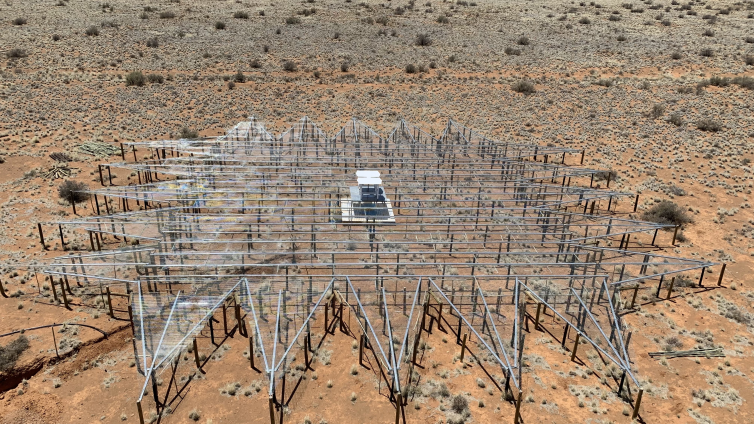
\includegraphics[width=0.6\textwidth]{images/antenna.png}
	\end{figure}

	\begin{center}
		\begin{tikzpicture}
			\node[draw, rounded corners, inner sep=10pt] (box) {%
				\begin{minipage}{0.9\textwidth} % Width of the box
					\begin{columns}[c] % Align columns centrally inside the box
						\begin{column}{0.33\textwidth}
							\centering
							{\small We measure \textit{sky averaged} signal.}
						\end{column}
						\begin{column}{0.33\textwidth}
							\centering
							{\small Antenna  LNA impedance mismatch}
						\end{column}
						\begin{column}{0.33\textwidth}
							\centering
							{\small Very faint signal.}
						\end{column}
					\end{columns}
				\end{minipage}
			};
		\end{tikzpicture}
	\end{center}

\end{frame}

\begin{frame}{\small{How to calibrate (in a bit more detail...)?}}
	\vspace{-0.5cm}
	\begin{flushleft}
		\textbf{Objective:} Map input temperature to output power.
		\vspace{0.2cm}

		\textbf{Key Factors:}
		\begin{itemize}
			\item LNA introduces time-dependent gain, $g(t)$.
			\item Impedance mismatch adds noise ($T_{\text{rec}}$) to the system.
		\end{itemize}

		\vspace{0.2cm}
		\textbf{Link Output Power to Input Temperature:}
	\end{flushleft}

	\begin{columns}
		\begin{column}{0.5\textwidth}
			{
				\begin{equation}
					P_{\text{out}}^{\text{src}} = g M \times \left( T_{\text{in}}^{\text{src}} + T_{\text{rec}} \right)
				\end{equation}
			}

		\end{column}
		\begin{column}{0.3\textwidth}

			\small $M = \left( 1 - |\Gamma_{\text{cal}}|^2 \right) | \frac{\sqrt{1 - |\Gamma_{\text{rec}}|^2}}{1 - \Gamma_{\text{cal}} \Gamma_{\text{rec}}}|^2$
		\end{column}
	\end{columns}

	\vfill

	\begin{footnotesize}
		\textit{Note: All parameters above are frequency-dependent, but the notation has been simplified here and thereafter for convenience.}
	\end{footnotesize}

\end{frame}


\begin{frame}{\small{Receiver/source mismatch}}
	\begin{figure}[h]
		\centering
		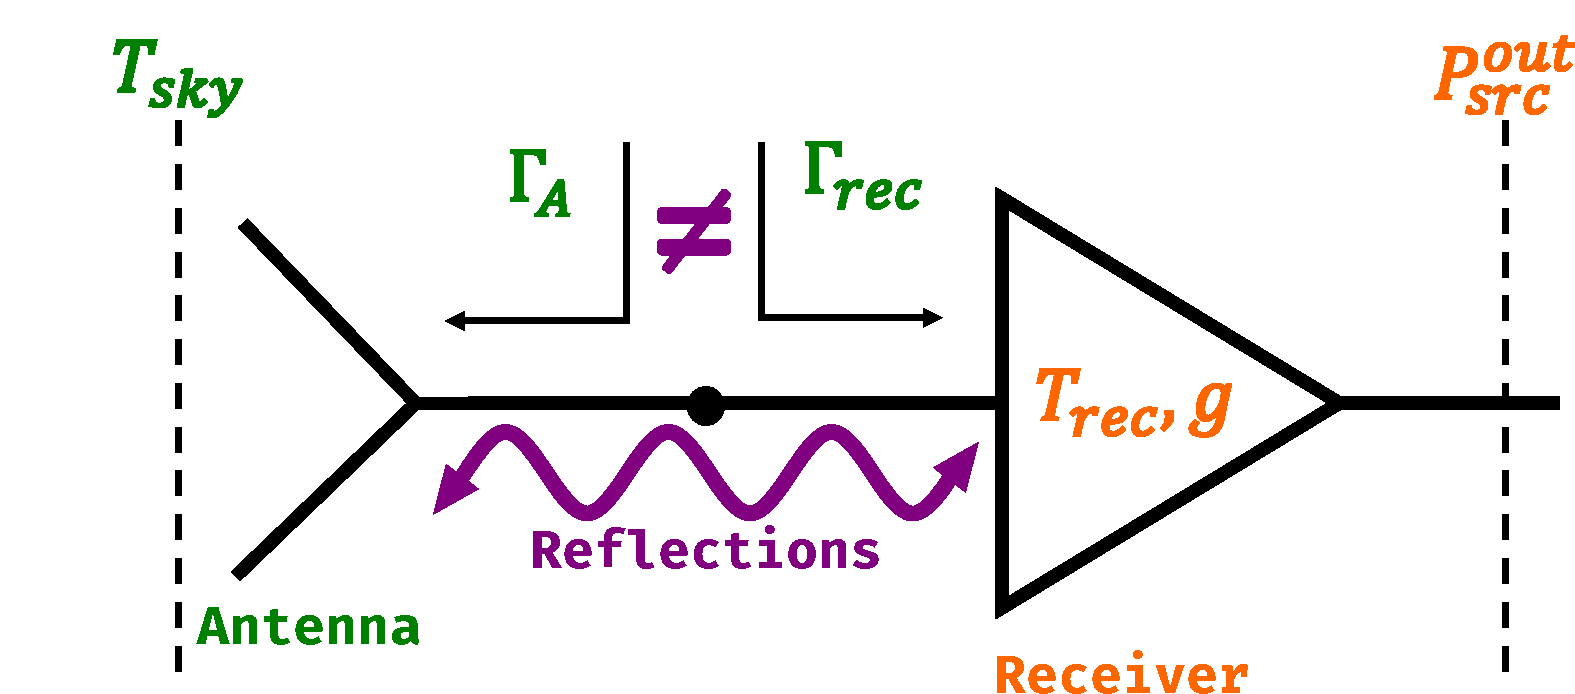
\includegraphics[width=0.9\textwidth]{images/intro_receiver.pdf}
		\caption{Schematic of the receiver system showing the signal path from antenna to digitizer}
	\end{figure}
\end{frame}

\begin{frame}{\small{Dealing with reflections...}}

	% Output Power Equation without title, maintaining the same equation number (1)
	\begin{minipage}{0.75\textwidth}
		{\tiny
			\begin{equation}
				P_{\text{out}}^{\text{src}} = \textcolor{red}{g} M \left( T_{\text{in}}^{\text{src}} + \textcolor{red}{T_{\text{rec}}} \right)
			\end{equation}
		}
	\end{minipage}

	\vspace{0.1cm}
	\hrule  % Horizontal line for separation
	\vspace{0.1cm}

	% Noise Parameter Equation with smaller, uniform title
	\begin{minipage}{0.75\textwidth}
		\textbf{\small{Noise Parameter Equation:}}
		{\tiny
			\begin{equation}
				P_{\text{out}}^{\text{src}} = \textcolor{red}{g} M \left( T_{\text{in}}^{\text{src}} + \textcolor{red}{T_{\text{min}}} + T_0 \frac{4\textcolor{red}{R_N}}{Z_0} \frac{|\Gamma_{\text{src}} - \textcolor{red}{\Gamma_{\text{opt}}}|^2}{(1 - |\Gamma_{\text{src}}|^2)(1 + |\Gamma_{\text{opt}}|^2)} \right)
			\end{equation}
		}
	\end{minipage}
	\quad
	\begin{minipage}{0.2\textwidth}
		\tiny
		\begin{itemize}
			\item \( g \) - Gain
			\item \( T_{\text{min}} \) - Minimum Noise Temperature
			\item \( R_N \) - Noise Resistance
			\item \( \Gamma_{\text{opt}} \) - Optimum Reflection Coefficient
		\end{itemize}
	\end{minipage}

	\vspace{0.05cm}
	\hrule  % Horizontal line for separation
	\vspace{0.05cm}

	% Noise Wave Equation with smaller, uniform title
	\begin{minipage}{0.75\textwidth}
		\textbf{\small{Noise Wave Equation:}}
		{\tiny
			\begin{multline}
				P_{\text{out}}^{\text{src}} = \textcolor{red}{g} \left[ \textcolor{red}{T_0} + \textcolor{red}{T_{\text{unc}}} |\Gamma_{\text{s}}|^2 \left|\frac{ \sqrt{1 - |\Gamma_{\text{rec}}|^2}}{1 - \Gamma_{\text{s}}\Gamma_{\text{rec}}} \right|^2 \right. \\
					\left. + T_{\text{s}}(1 - |\Gamma_{\text{s}}|^2) \left|\frac{ \sqrt{1 - |\Gamma_{\text{rec}}|^2}}{1 - \Gamma_{\text{s}}\Gamma_{\text{rec}}} \right|^2 + \textcolor{red}{T_{\text{cos}}} \Re \left( \Gamma_{\text{s}} \frac{\sqrt{1 - |\Gamma_{\text{rec}}|^2}}{1 - \Gamma_{\text{s}} \Gamma_{\text{rec}}} \right) \right. \\
					\left. + \textcolor{red}{T_{\text{sin}}} \Im \left( \Gamma_{\text{s}} \frac{\sqrt{1 - |\Gamma_{\text{rec}}|^2}}{1 - \Gamma_{\text{s}} \Gamma_{\text{rec}}} \right) \right]
			\end{multline}
		}
	\end{minipage}
	\quad
	\begin{minipage}{0.2\textwidth}
		\tiny
		\begin{itemize}
			\item \( \Gamma_{\text{s}} \) - Source Reflection Coefficient
			\item \( \Gamma_{\text{rec}} \) - Receiver Reflection Coefficient
			\item \( T_{\text{s}} \) - Source Temperature
			\item $P_{\text{out}}^{\text{src}}$ - Power out
			\item $T_{\text{unc, cos, sin}}$ - Noise wave parameters
			\item $T_{0}$ reference temperature
		\end{itemize}
	\end{minipage}

\end{frame}
\section{Radiometer calibration with machine learning}
\begin{frame}{\small{Machine learning}}
	\begin{columns}
		\begin{column}{0.35\textwidth}
			\textbf{How/why?}
			\begin{itemize}
				\item Can predict noise wave parameters using machine learning.
				\item Could apply method to noise parameters.
				\item Predict \textbf{directly} on noise parameters on frequency by frequency basis.
				\item Maleable to environmental changes.
			\end{itemize}
		\end{column}
		\begin{column}{0.65\textwidth}
			\begin{figure}[h]
				\includesvg[width=0.9\textwidth]{images/mlcal.svg}
			\end{figure}
		\end{column}
	\end{columns}
\end{frame}


\begin{frame}{\small{Machine learning calibration steps}}
	\footnotesize
	\begin{columns}
		% Left Column: Steps 1 and 2
		\begin{column}{0.5\textwidth}
			\textbf{1. Define the Loss Function}\\
			Regress over measured power and predicted power.\\
			\begin{equation}
				\mathcal{L} = \frac{1}{n}\sum_{i=1}^{n} \left( \mathcal{P}_{\text{measured},i} - \mathcal{P}_{\text{pred},i} \right)^{2}
			\end{equation}

			\vspace{0.5cm} % Adds vertical space between steps

			\textbf{2. Write Down the Equation for \(\mathcal{P}_{\text{pred}}\)}\\
			Using the noise wave formalism, relate \(\mathcal{P}_{\text{pred}}\) to \(T_{\text{src}}\).
			\begin{align}
				 & \mathcal{P}_{\text{pred}} = \textcolor{red}{g} \cdot M \left( T_{\text{in}}^{\text{src}} \right. \nonumber                                                                                                               \\
				 & \quad + \textcolor{red}{T_{\text{min}}} + T_0 \frac{4\textcolor{red}{R_N}}{Z_0} \frac{|\Gamma_{\text{src}} - \textcolor{red}{\Gamma_{\text{opt}}}|^2}{(1 - |\Gamma_{\text{src}}|^2)(1 + |\Gamma_{\text{opt}}|^2)} \Bigg)
			\end{align}
			\vfill
		\end{column}

		% Right Column: Step 3 with Definitions of Theta
		\begin{column}{0.5\textwidth}
			\textbf{3. Minimise the Loss Function}
			\begin{equation}
				\boldsymbol{\theta}^* = \arg\min_{\boldsymbol{\theta}} \mathcal{L}(\boldsymbol{\theta})
			\end{equation}
			parameter vector \(\boldsymbol{\theta}\) includes all tunable parameters in the model:
			\begin{equation}
				\boldsymbol{\theta} = \{ \textcolor{red}{g}, \textcolor{red}{T_{\text{min}}}, \textcolor{red}{R_N}, \textcolor{red}{\Gamma_{\text{opt}}^{\phi}}, \textcolor{red}{|\Gamma_{\text{opt}}|)}
			\end{equation}

			\textbf{4. Rearrange and Predict $(T_{\text{src}}$) using $\boldsymbol{\theta}^{*}$}
			\begin{align}
				T_{\text{src}} & = \frac{\mathcal{P}_{\text{pred}}}{\textcolor{red}{g^*} \cdot M} \nonumber \\
				               & \quad - \left( \textcolor{red}{T_{\text{min}}^*}
				+ T_0 \frac{4\textcolor{red}{R_N^*}}{Z_0} \frac{|\Gamma_{\text{src}} - \textcolor{red}{\Gamma_{\text{opt}}^*}|^2}{(1 - |\Gamma_{\text{src}}|^2)(1 + |\Gamma_{\text{opt}}^*|^2)} \right)
			\end{align}
			\vfill
		\end{column}
	\end{columns}
\end{frame}

\begin{frame}{\small{ML calibration overview}}
	\begin{figure}[h]
		\centering
		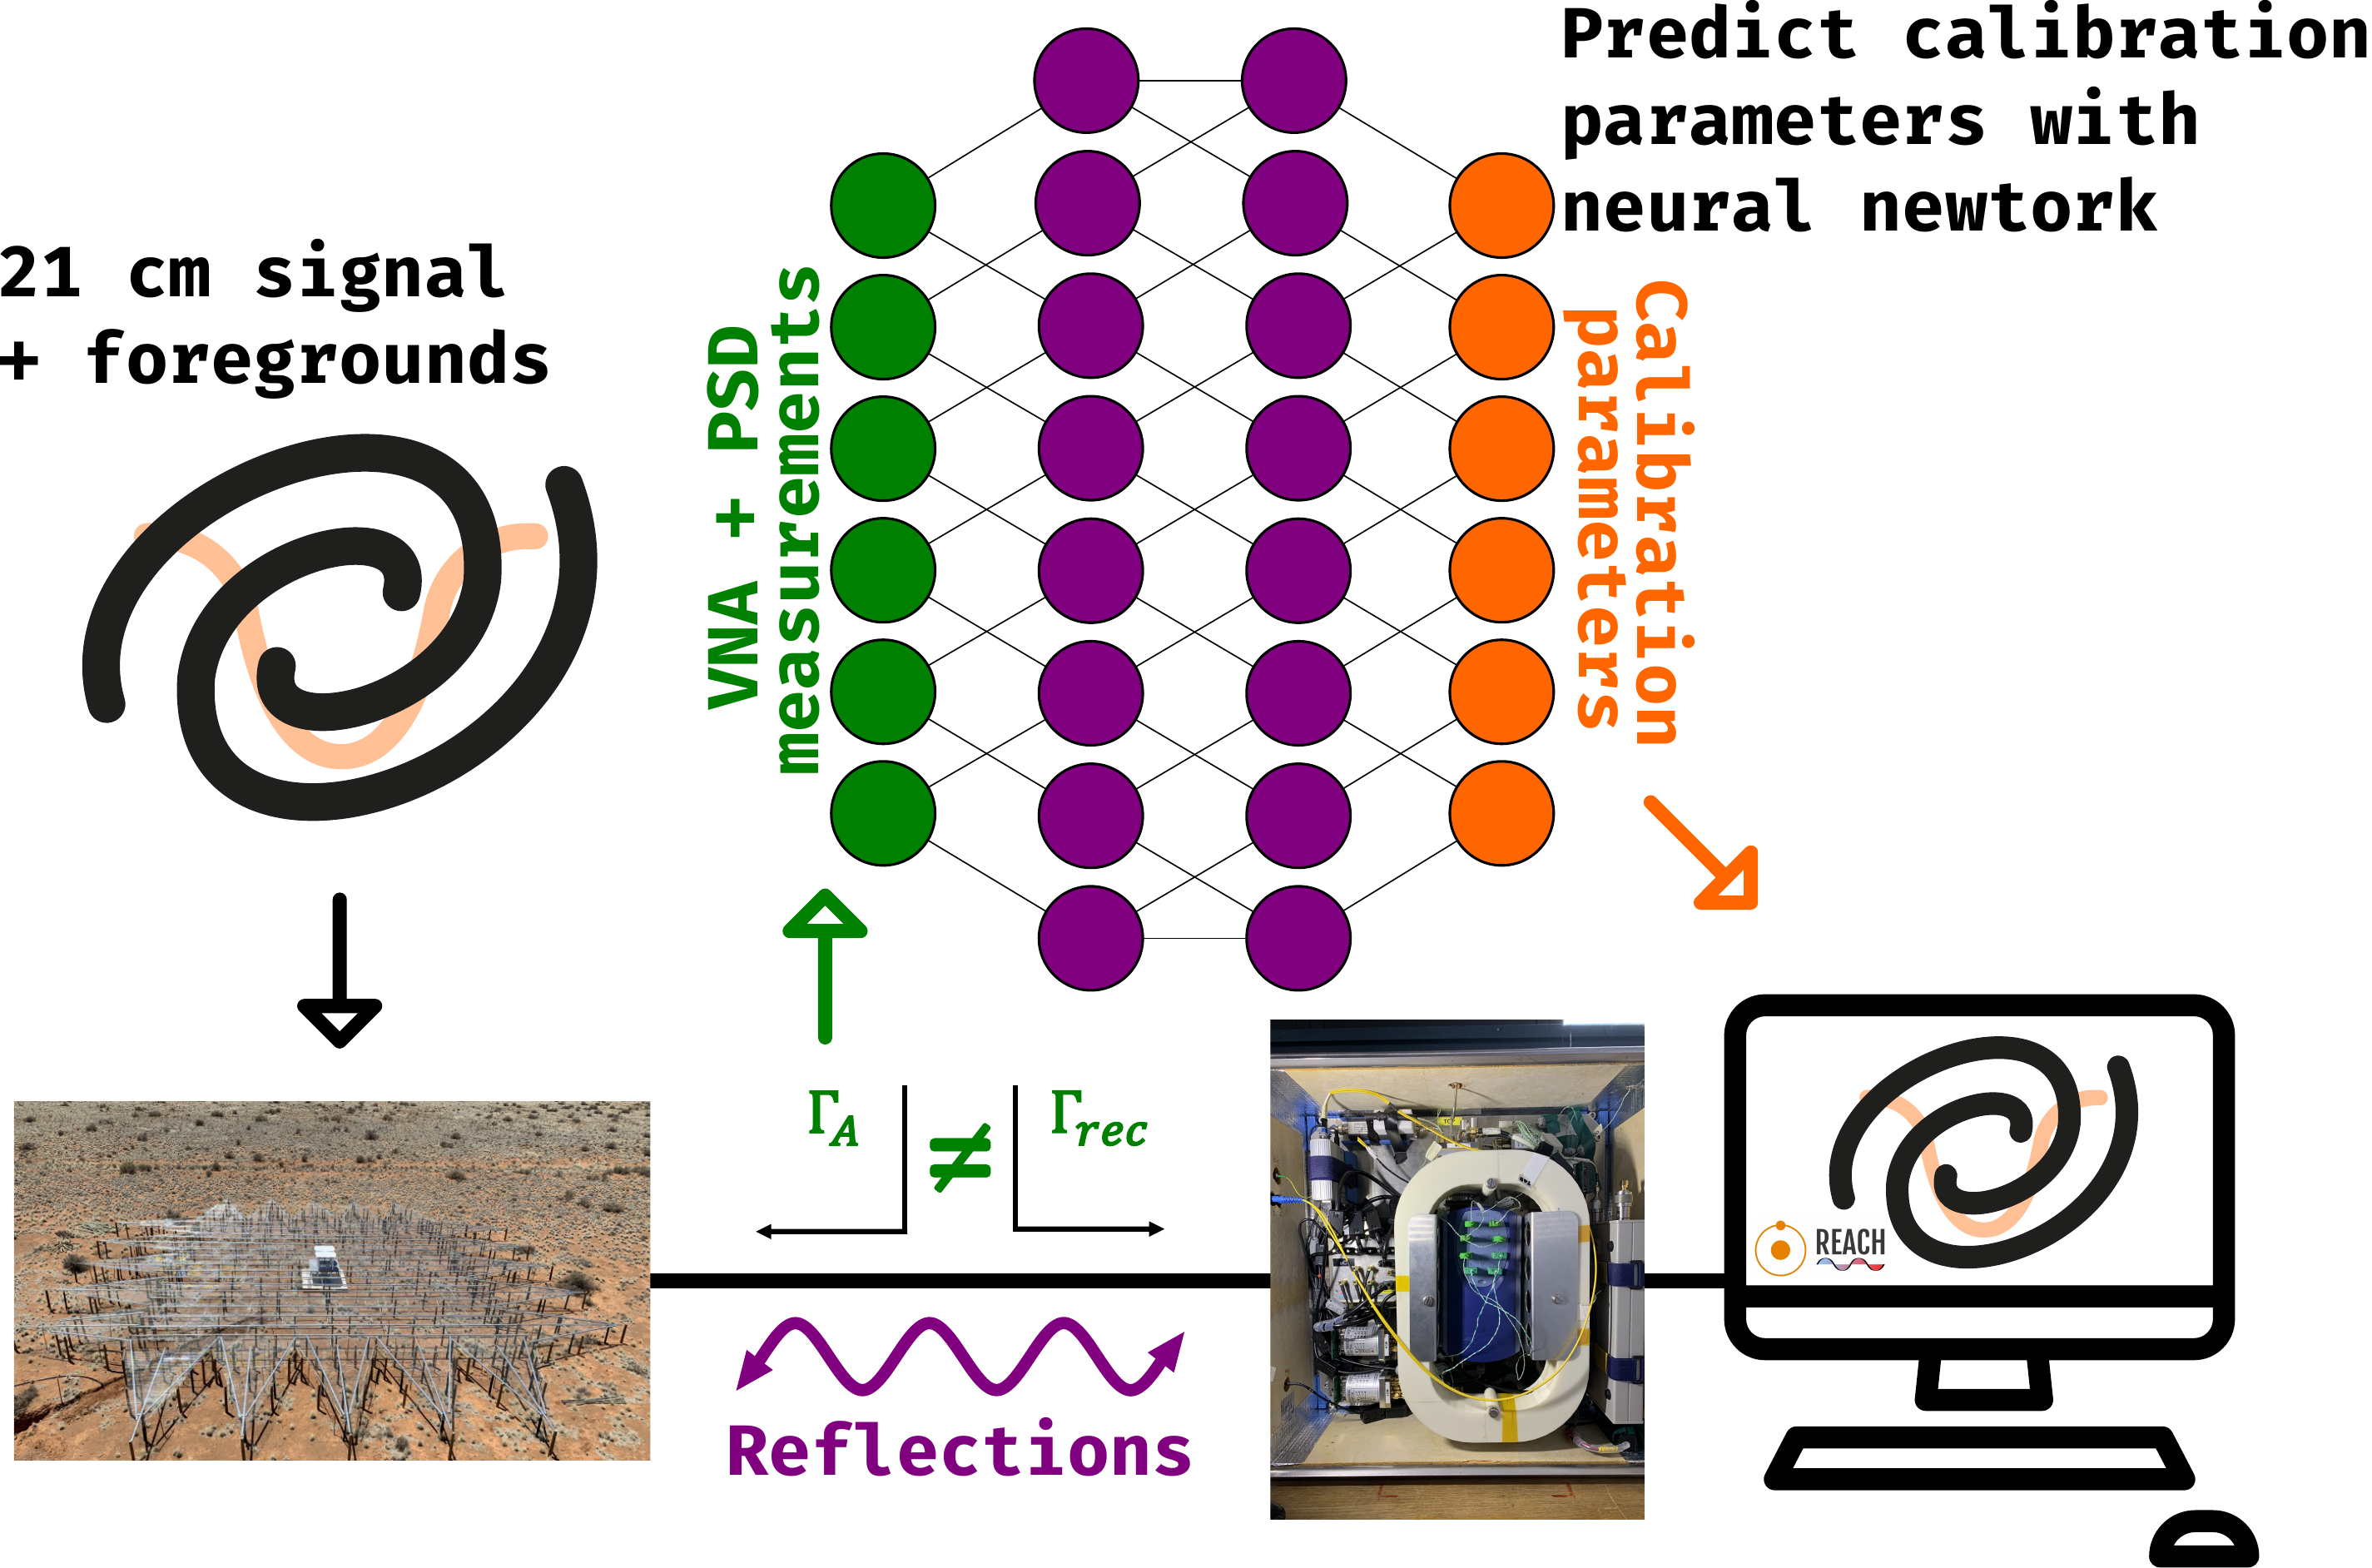
\includegraphics[width=0.6\textwidth]{images/ml_overview.pdf}
		\caption{High-level overview of the machine learning-based calibration framework}
	\end{figure}
\end{frame}

\begin{frame}{\small{The physical system}}
	\begin{columns}
		\begin{column}{0.3\textwidth}
			\textbf{Process:}
			\begin{itemize}
				\item Switch between sources to generate training data.
				\item Calibration sources with known temperature train neural net.
				\item Predict $T_{\text{src}}$ of antenna.
			\end{itemize}
		\end{column}

		\begin{column}{0.7\textwidth}
			\begin{figure}
				\centering
				\includesvg[width=\textwidth]{images/instrument.svg}
			\end{figure}
		\end{column}
	\end{columns}
	\vfill
\end{frame}

\begin{frame}{\small{Network Architecture}}
	\begin{columns}
		\begin{column}{0.35\textwidth}
			\textbf{Structure:}
			\begin{itemize}
				\item Input thermistor and VNA measurments.
				\item Also input frequency.
				\item Predict noise parameters.
				\item Regress over loss function.
			\end{itemize}
		\end{column}

		\begin{column}{0.65\textwidth}
			\begin{figure}
				\centering
				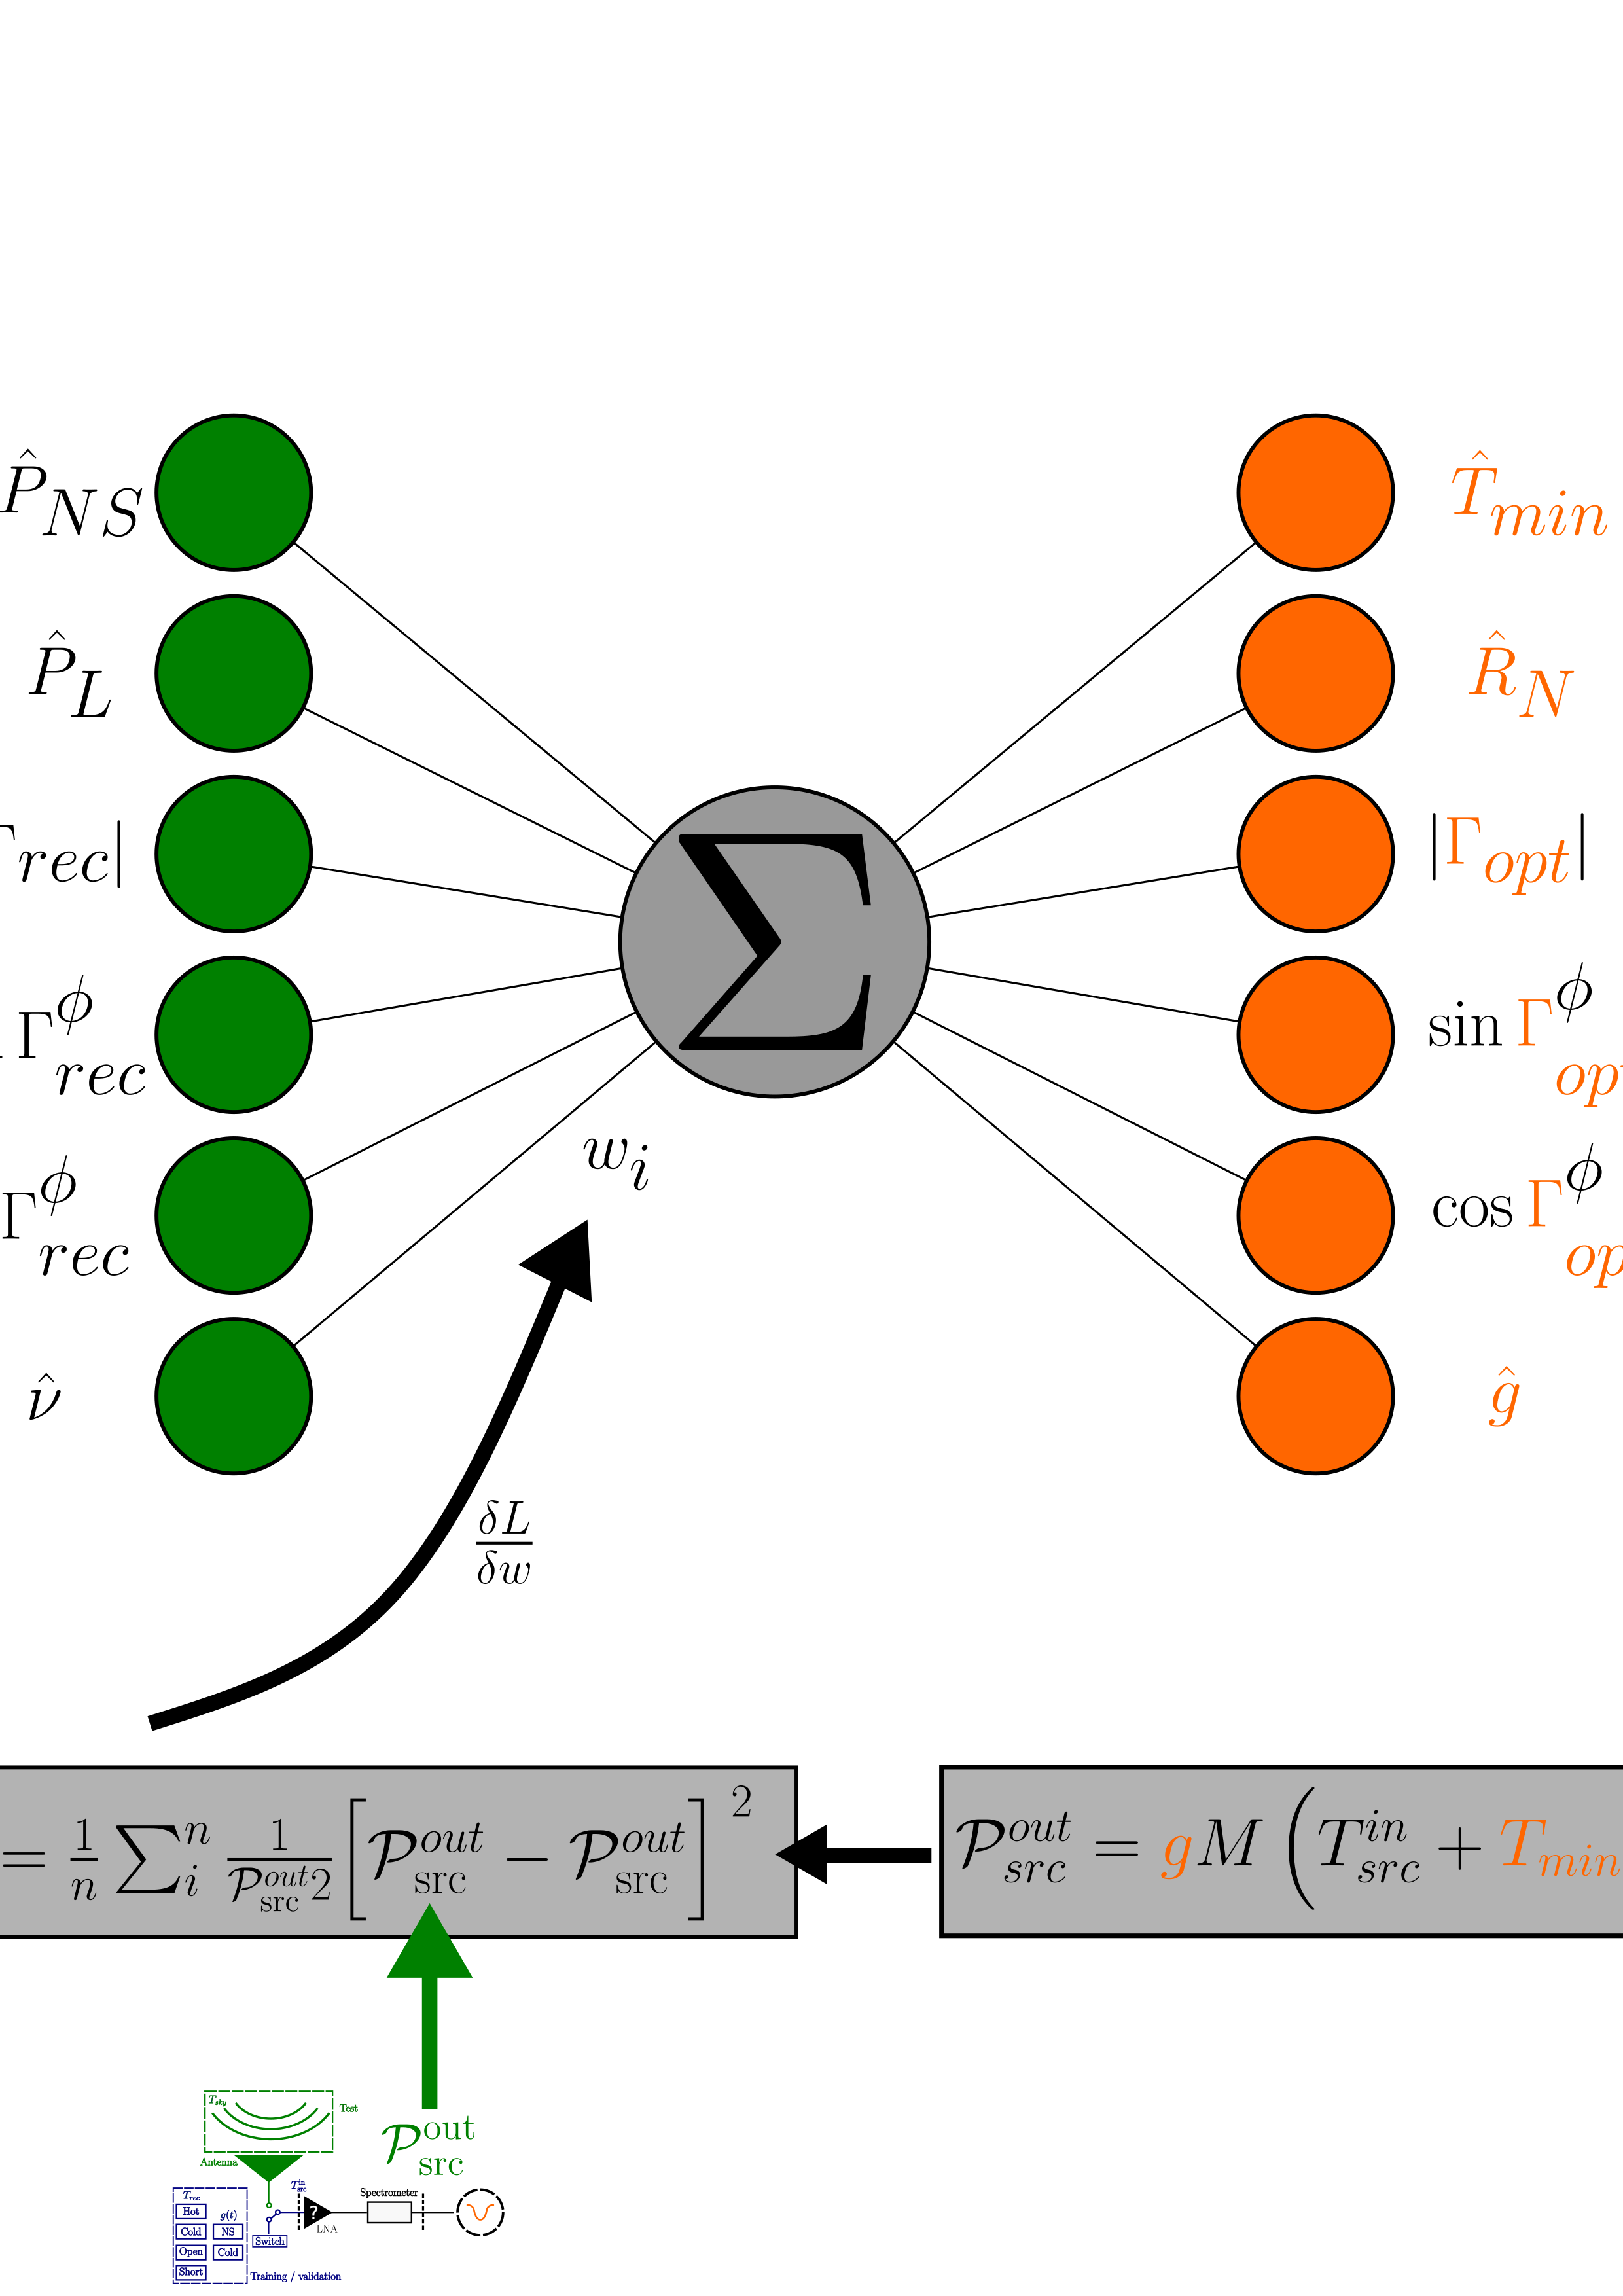
\includegraphics[width=0.75\textwidth]{images/nn.png}
			\end{figure}
		\end{column}
	\end{columns}
	\vfill
\end{frame}


\begin{frame}{\small{Testing on internal validation source}}
	\begin{figure}
		\centering
		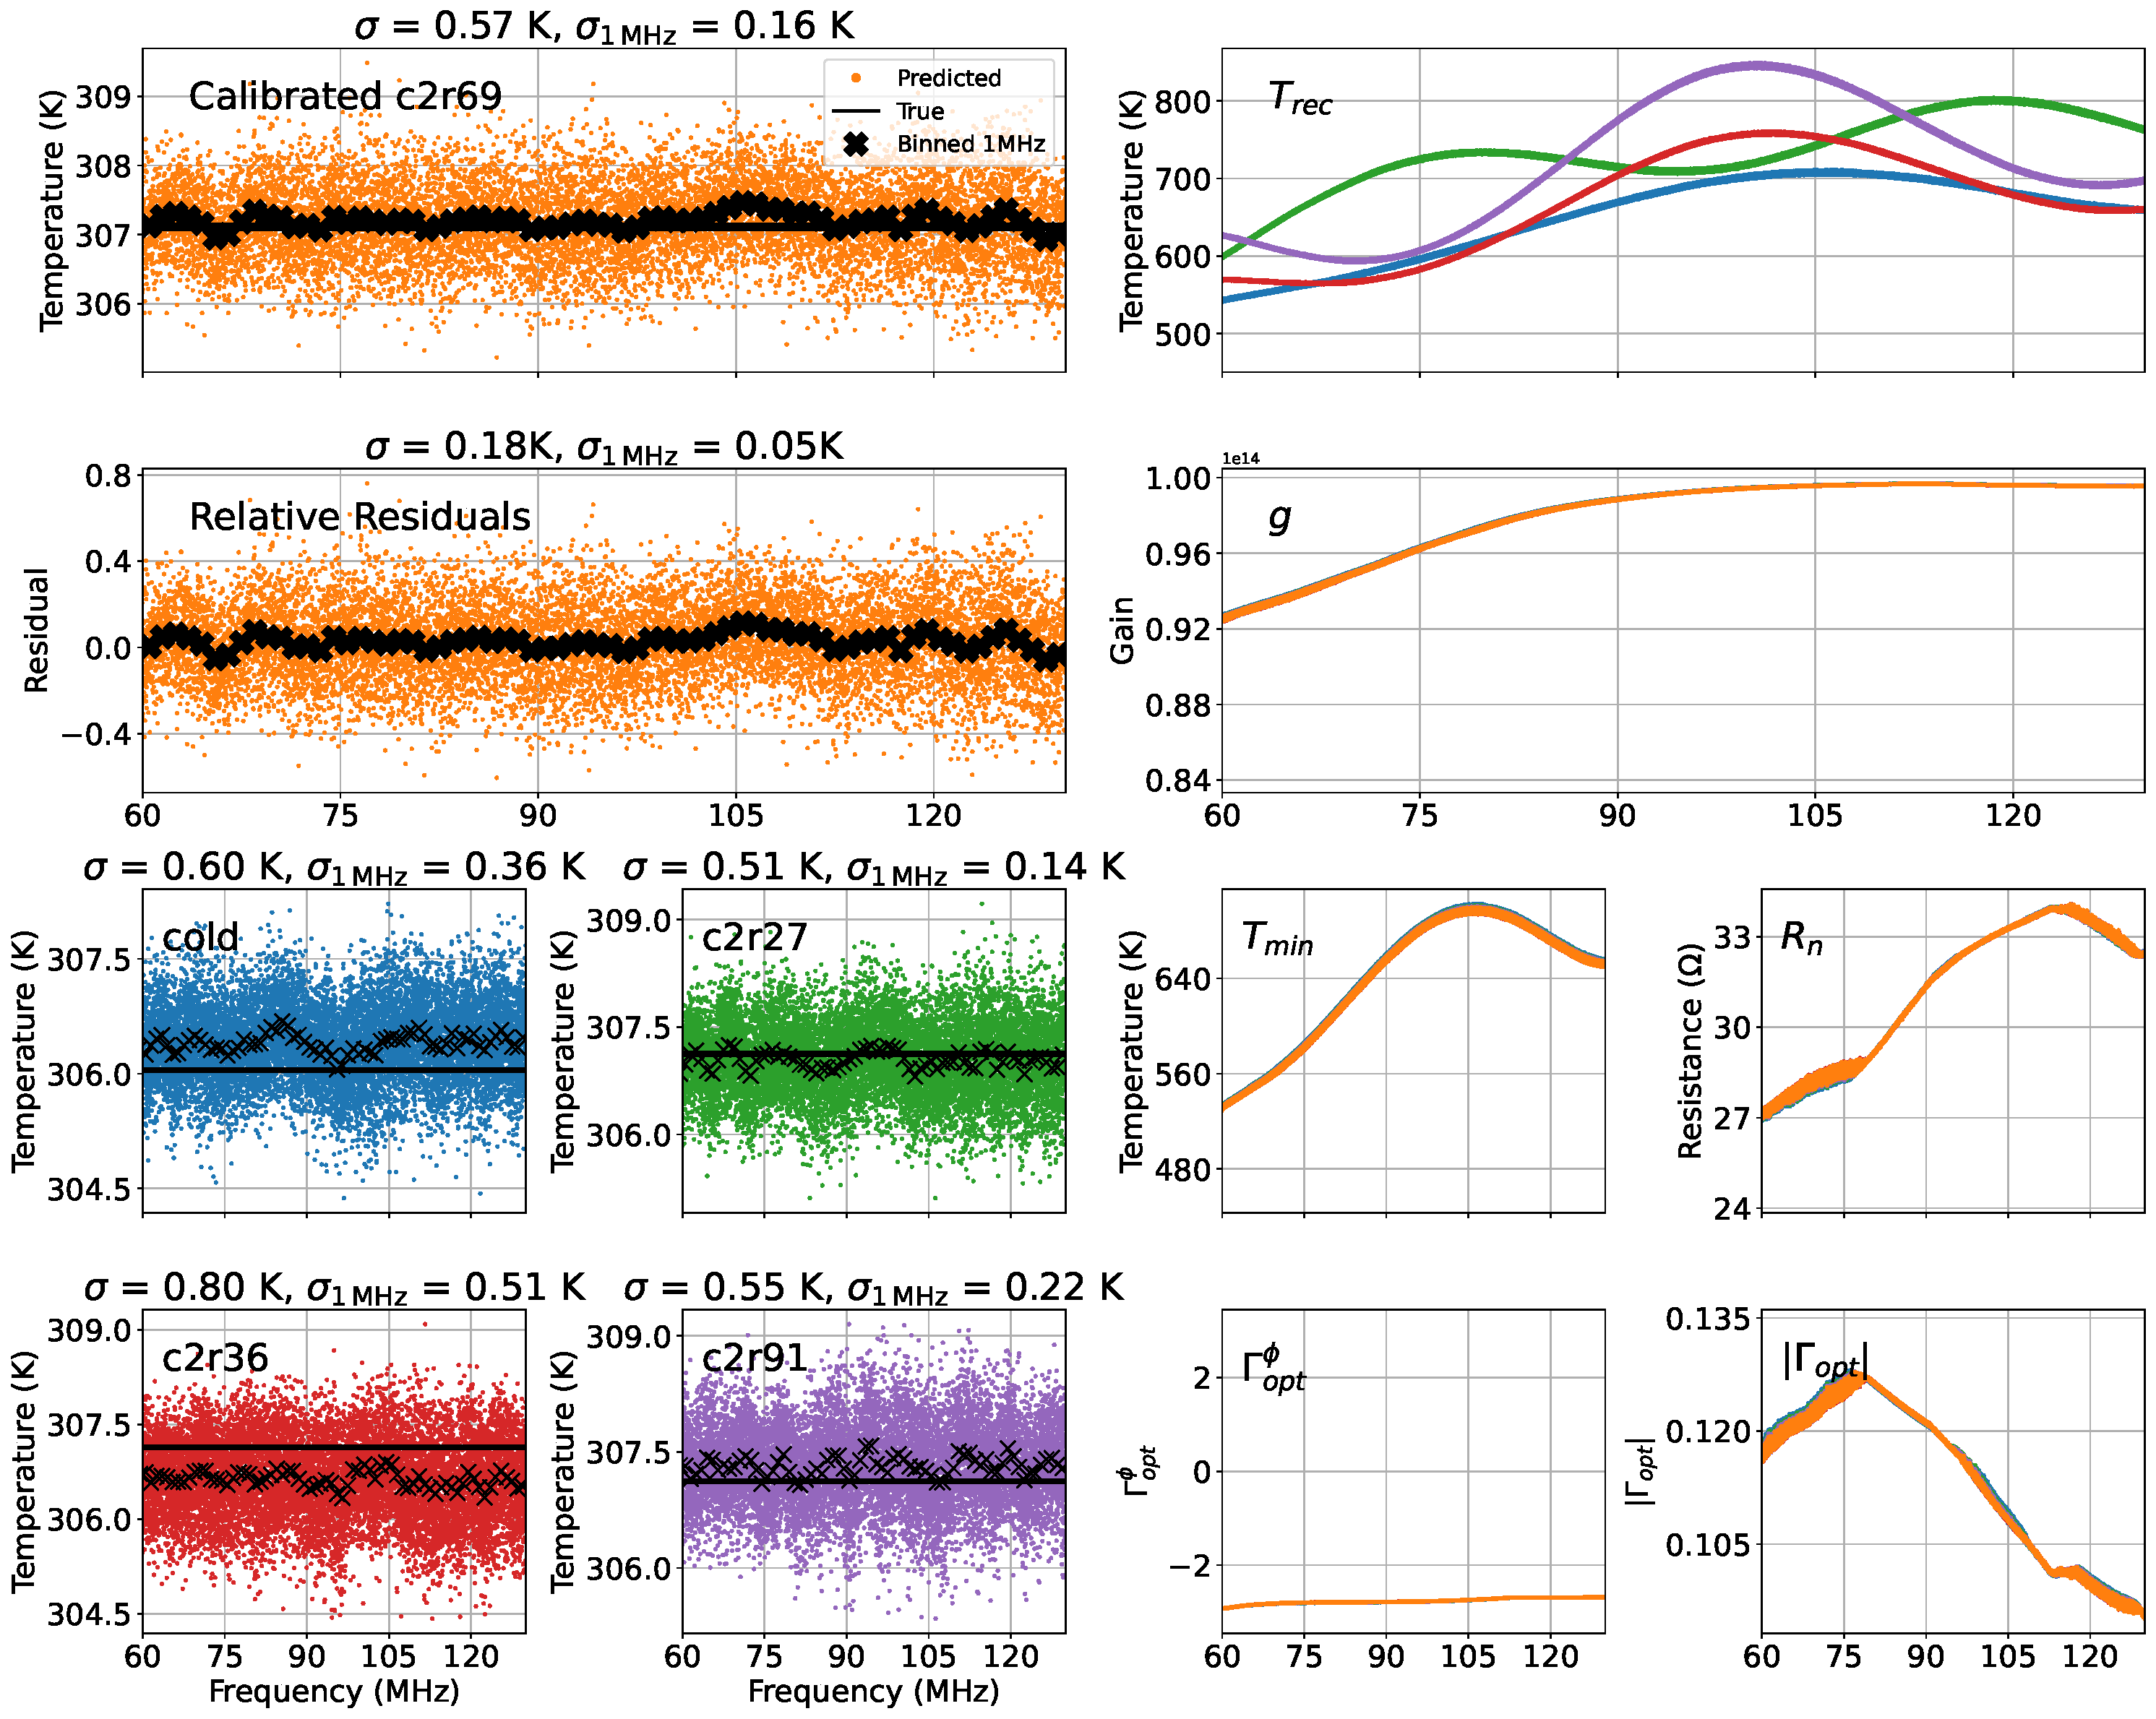
\includegraphics[width=0.55\textwidth]{images/temps.pdf}
		\caption{Temperature calibration using internal sources on the REACH receiver}
	\end{figure}
\end{frame}

\begin{frame}{\small{Does not require cable/switch corrections?}}
	\begin{columns}
		\begin{column}{0.5\textwidth}
			\begin{figure}
				\centering
				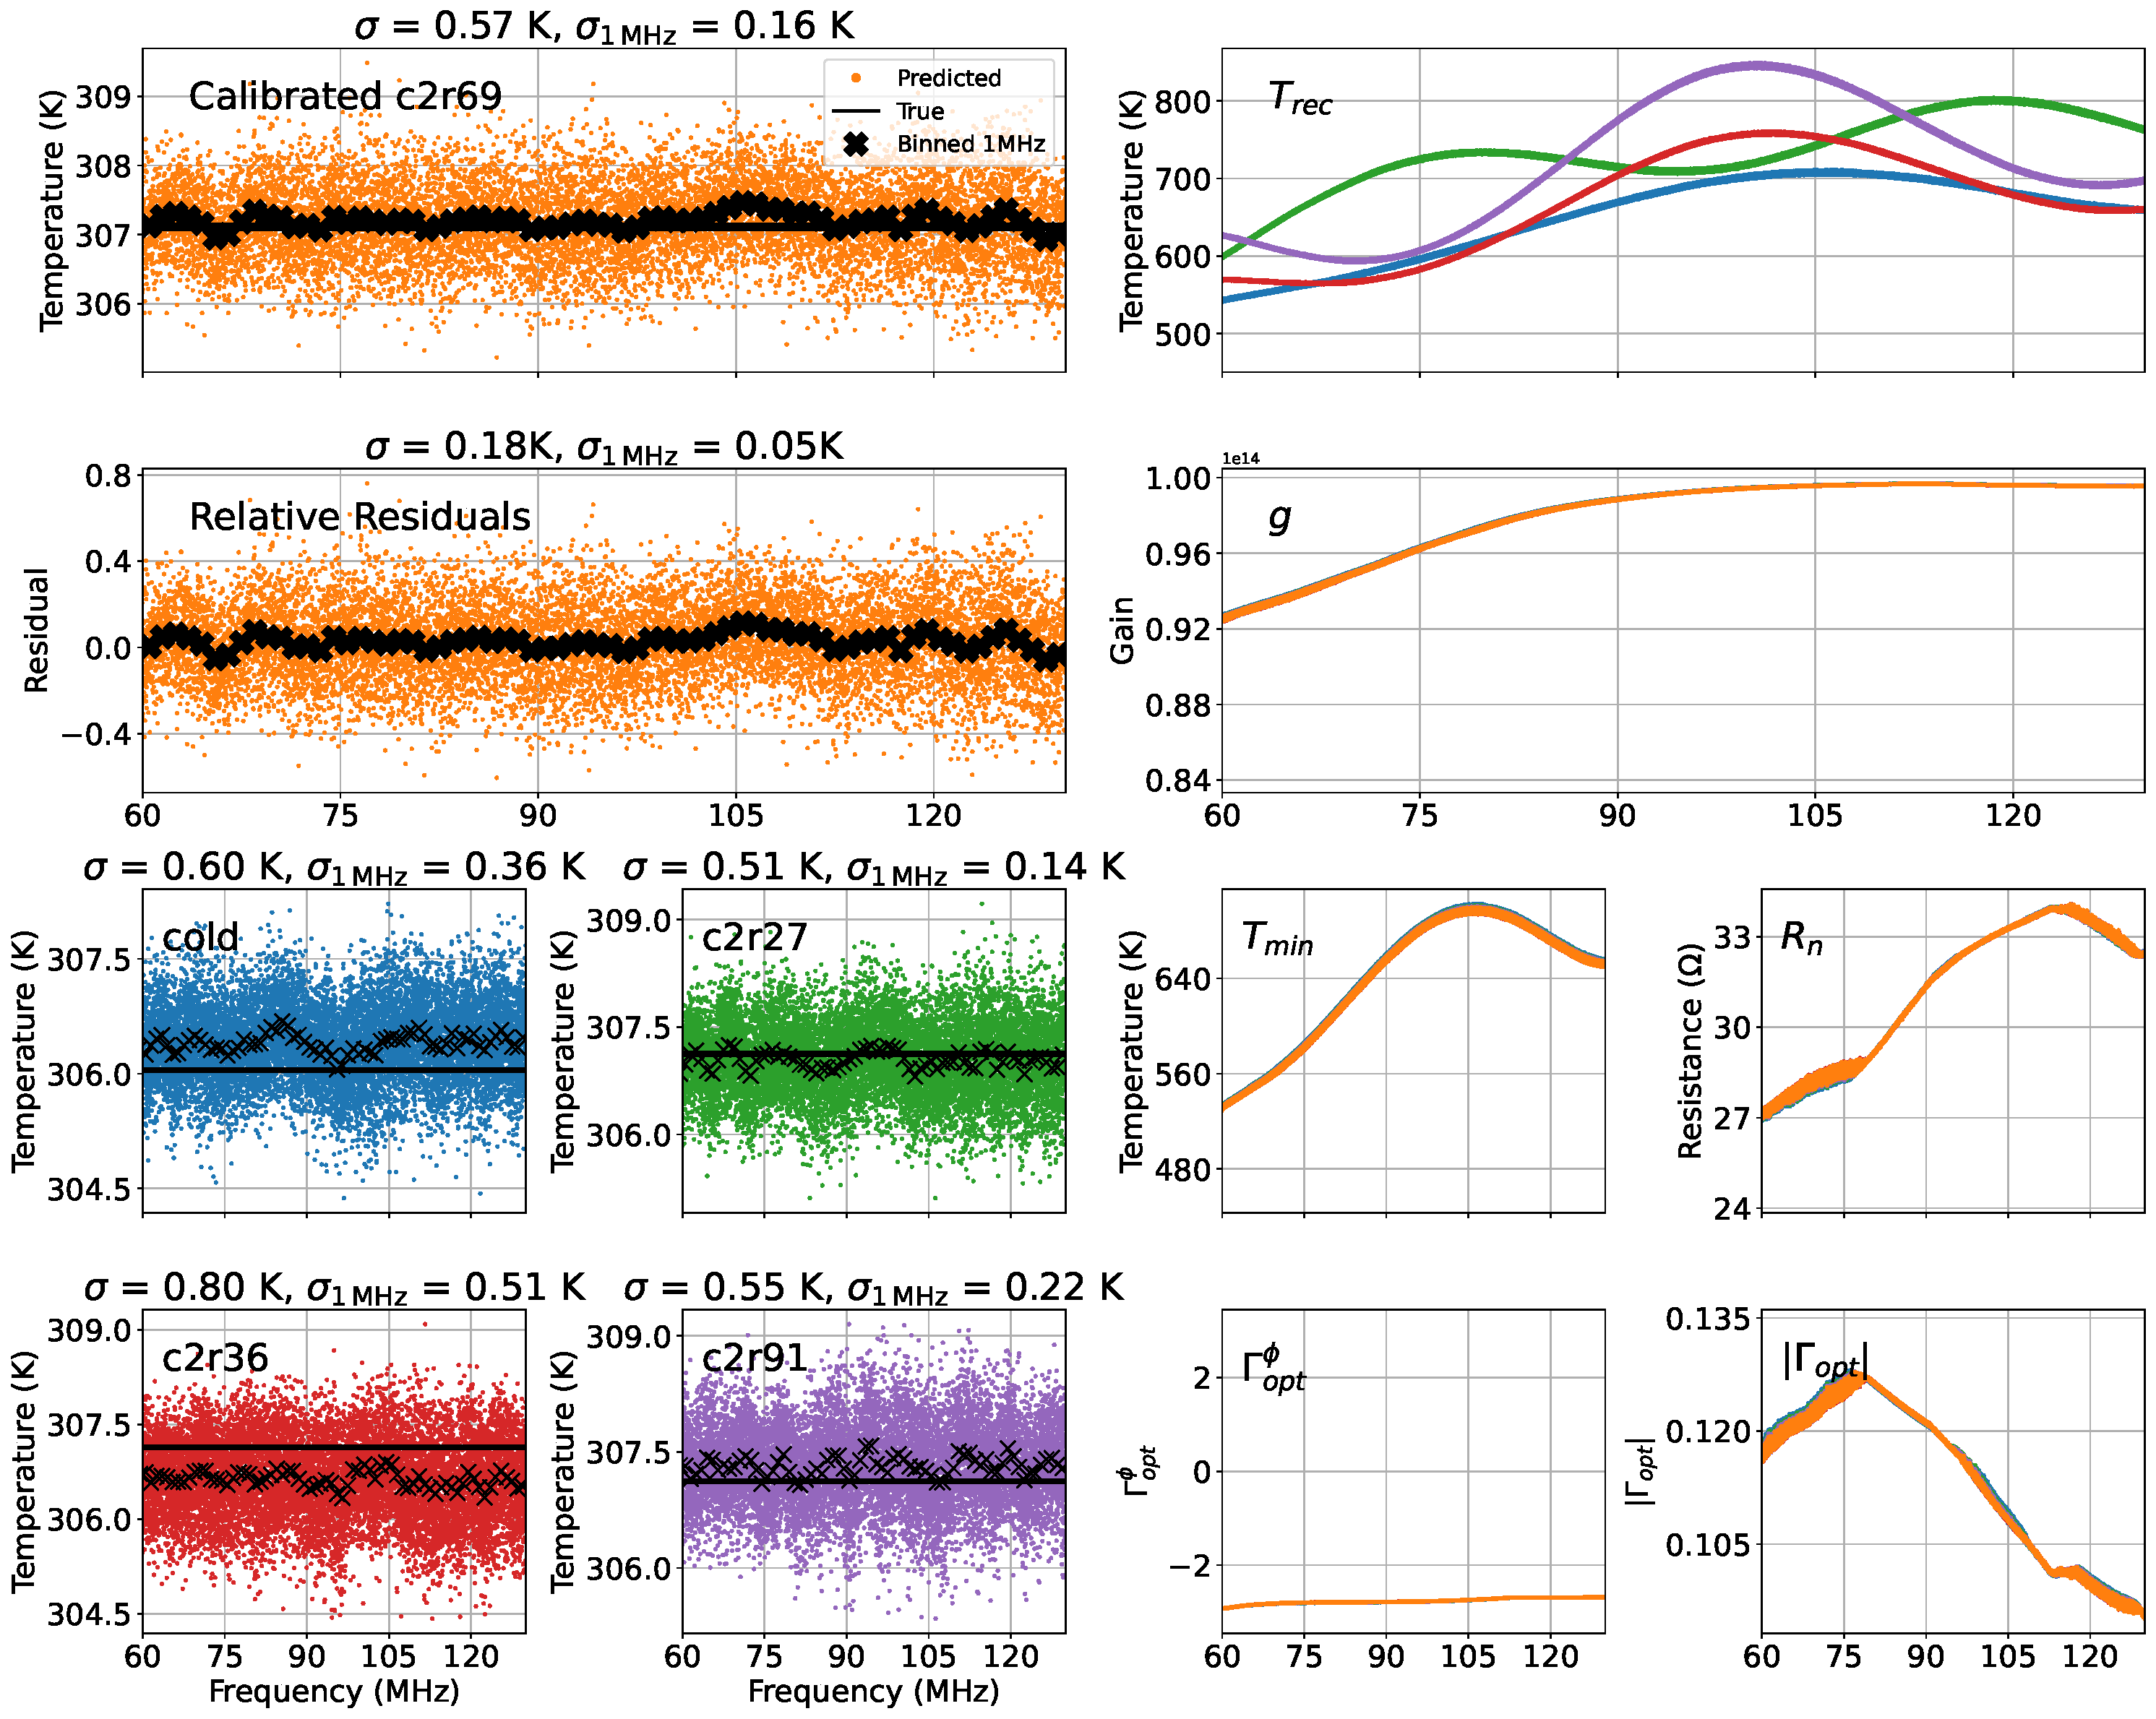
\includegraphics[width=0.9\textwidth]{images/temps.pdf}
			\end{figure}
		\end{column}
		\begin{column}{0.5\textwidth}
			\begin{figure}
				\centering
				\includesvg[width=0.9\textwidth]{images/instrument.svg}
			\end{figure}
		\end{column}
	\end{columns}
\end{frame}

\section{End to end 21cm experiment simulation}

\begin{frame}{\small{Simulation pipeline for radiometer calibration}}
	\begin{figure}
		\centering
		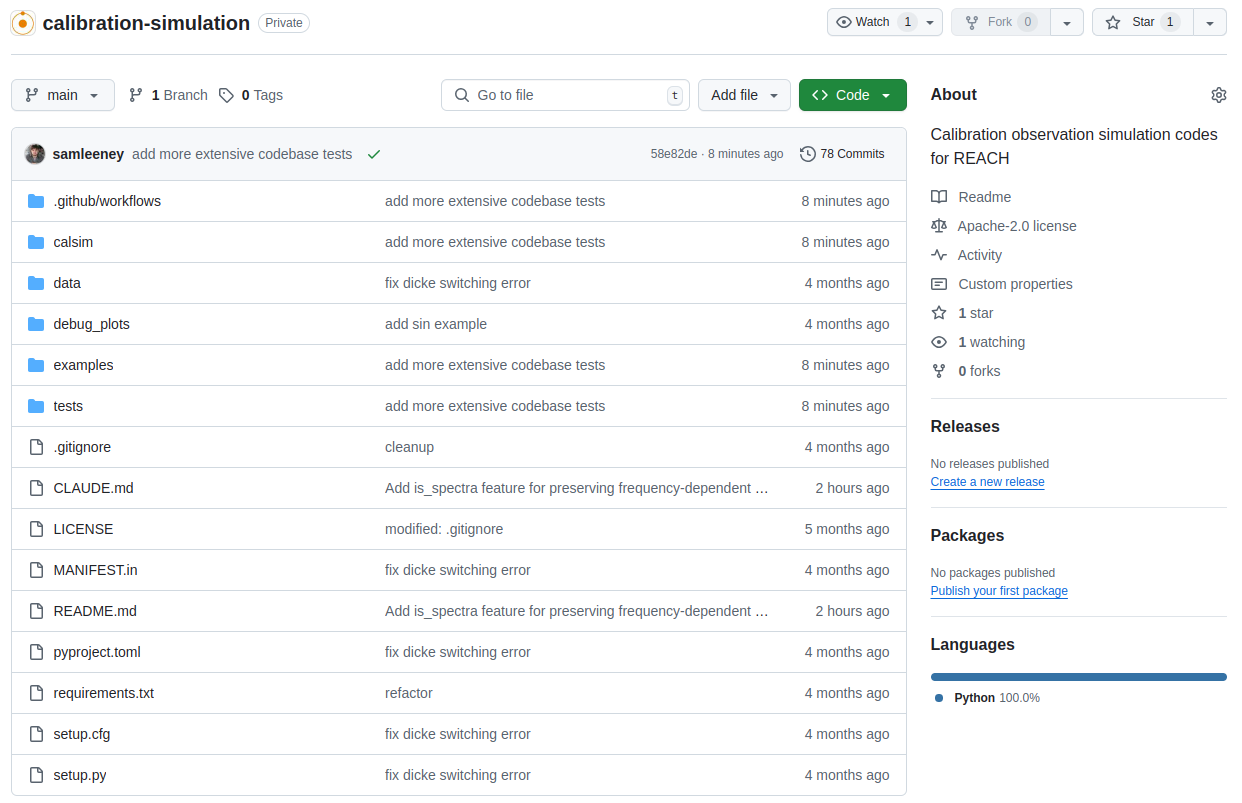
\includegraphics[width=0.7\textwidth]{images/githubrepo.png}
	\end{figure}
\end{frame}

\begin{frame}{\small{End to end simulation}}
	\vspace{-0.3cm}
	\begin{tcolorbox}[colback=blue!5!white,colframe=blue!75!black,title=]
		We have shown we can calibrate an internal source, we now test the
        method on as part of the broader system (simulated).
	\end{tcolorbox}
	\vspace{-0.3cm}
	\begin{figure}[h]
		\centering
		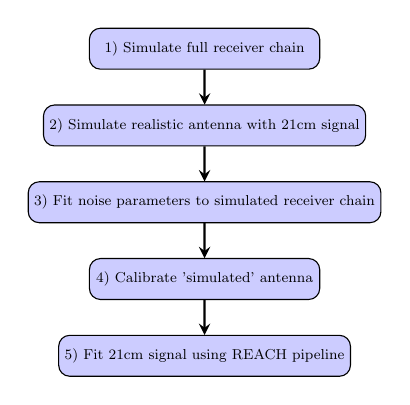
\begin{tikzpicture}[scale=0.65, transform shape]
			% Define styles
			\tikzstyle{process} = [rectangle, rounded corners, minimum width=4.5cm, minimum height=0.8cm, text centered, draw=black, fill=blue!20, font=\footnotesize]
			\tikzstyle{arrow} = [thick,->,>=stealth]
			
			% Nodes
			\node (step1) [process] at (0,0) {1) Simulate full receiver chain};
			\node (step2) [process] at (0,-1.5) {2) Simulate realistic antenna with 21cm signal};
			\node (step3) [process] at (0,-3) {3) Fit noise parameters to simulated receiver chain};
			\node (step4) [process] at (0,-4.5) {4) Calibrate 'simulated' antenna};
			\node (step5) [process] at (0,-6) {5) Fit 21cm signal using REACH pipeline};
			
			% Arrows
			\draw [arrow] (step1) -- (step2);
			\draw [arrow] (step2) -- (step3);
			\draw [arrow] (step3) -- (step4);
			\draw [arrow] (step4) -- (step5);
		\end{tikzpicture}
	\end{figure}
\end{frame}

\begin{frame}{\small{Predicted vs True Antenna Temperature}}
	\begin{figure}
		\centering
		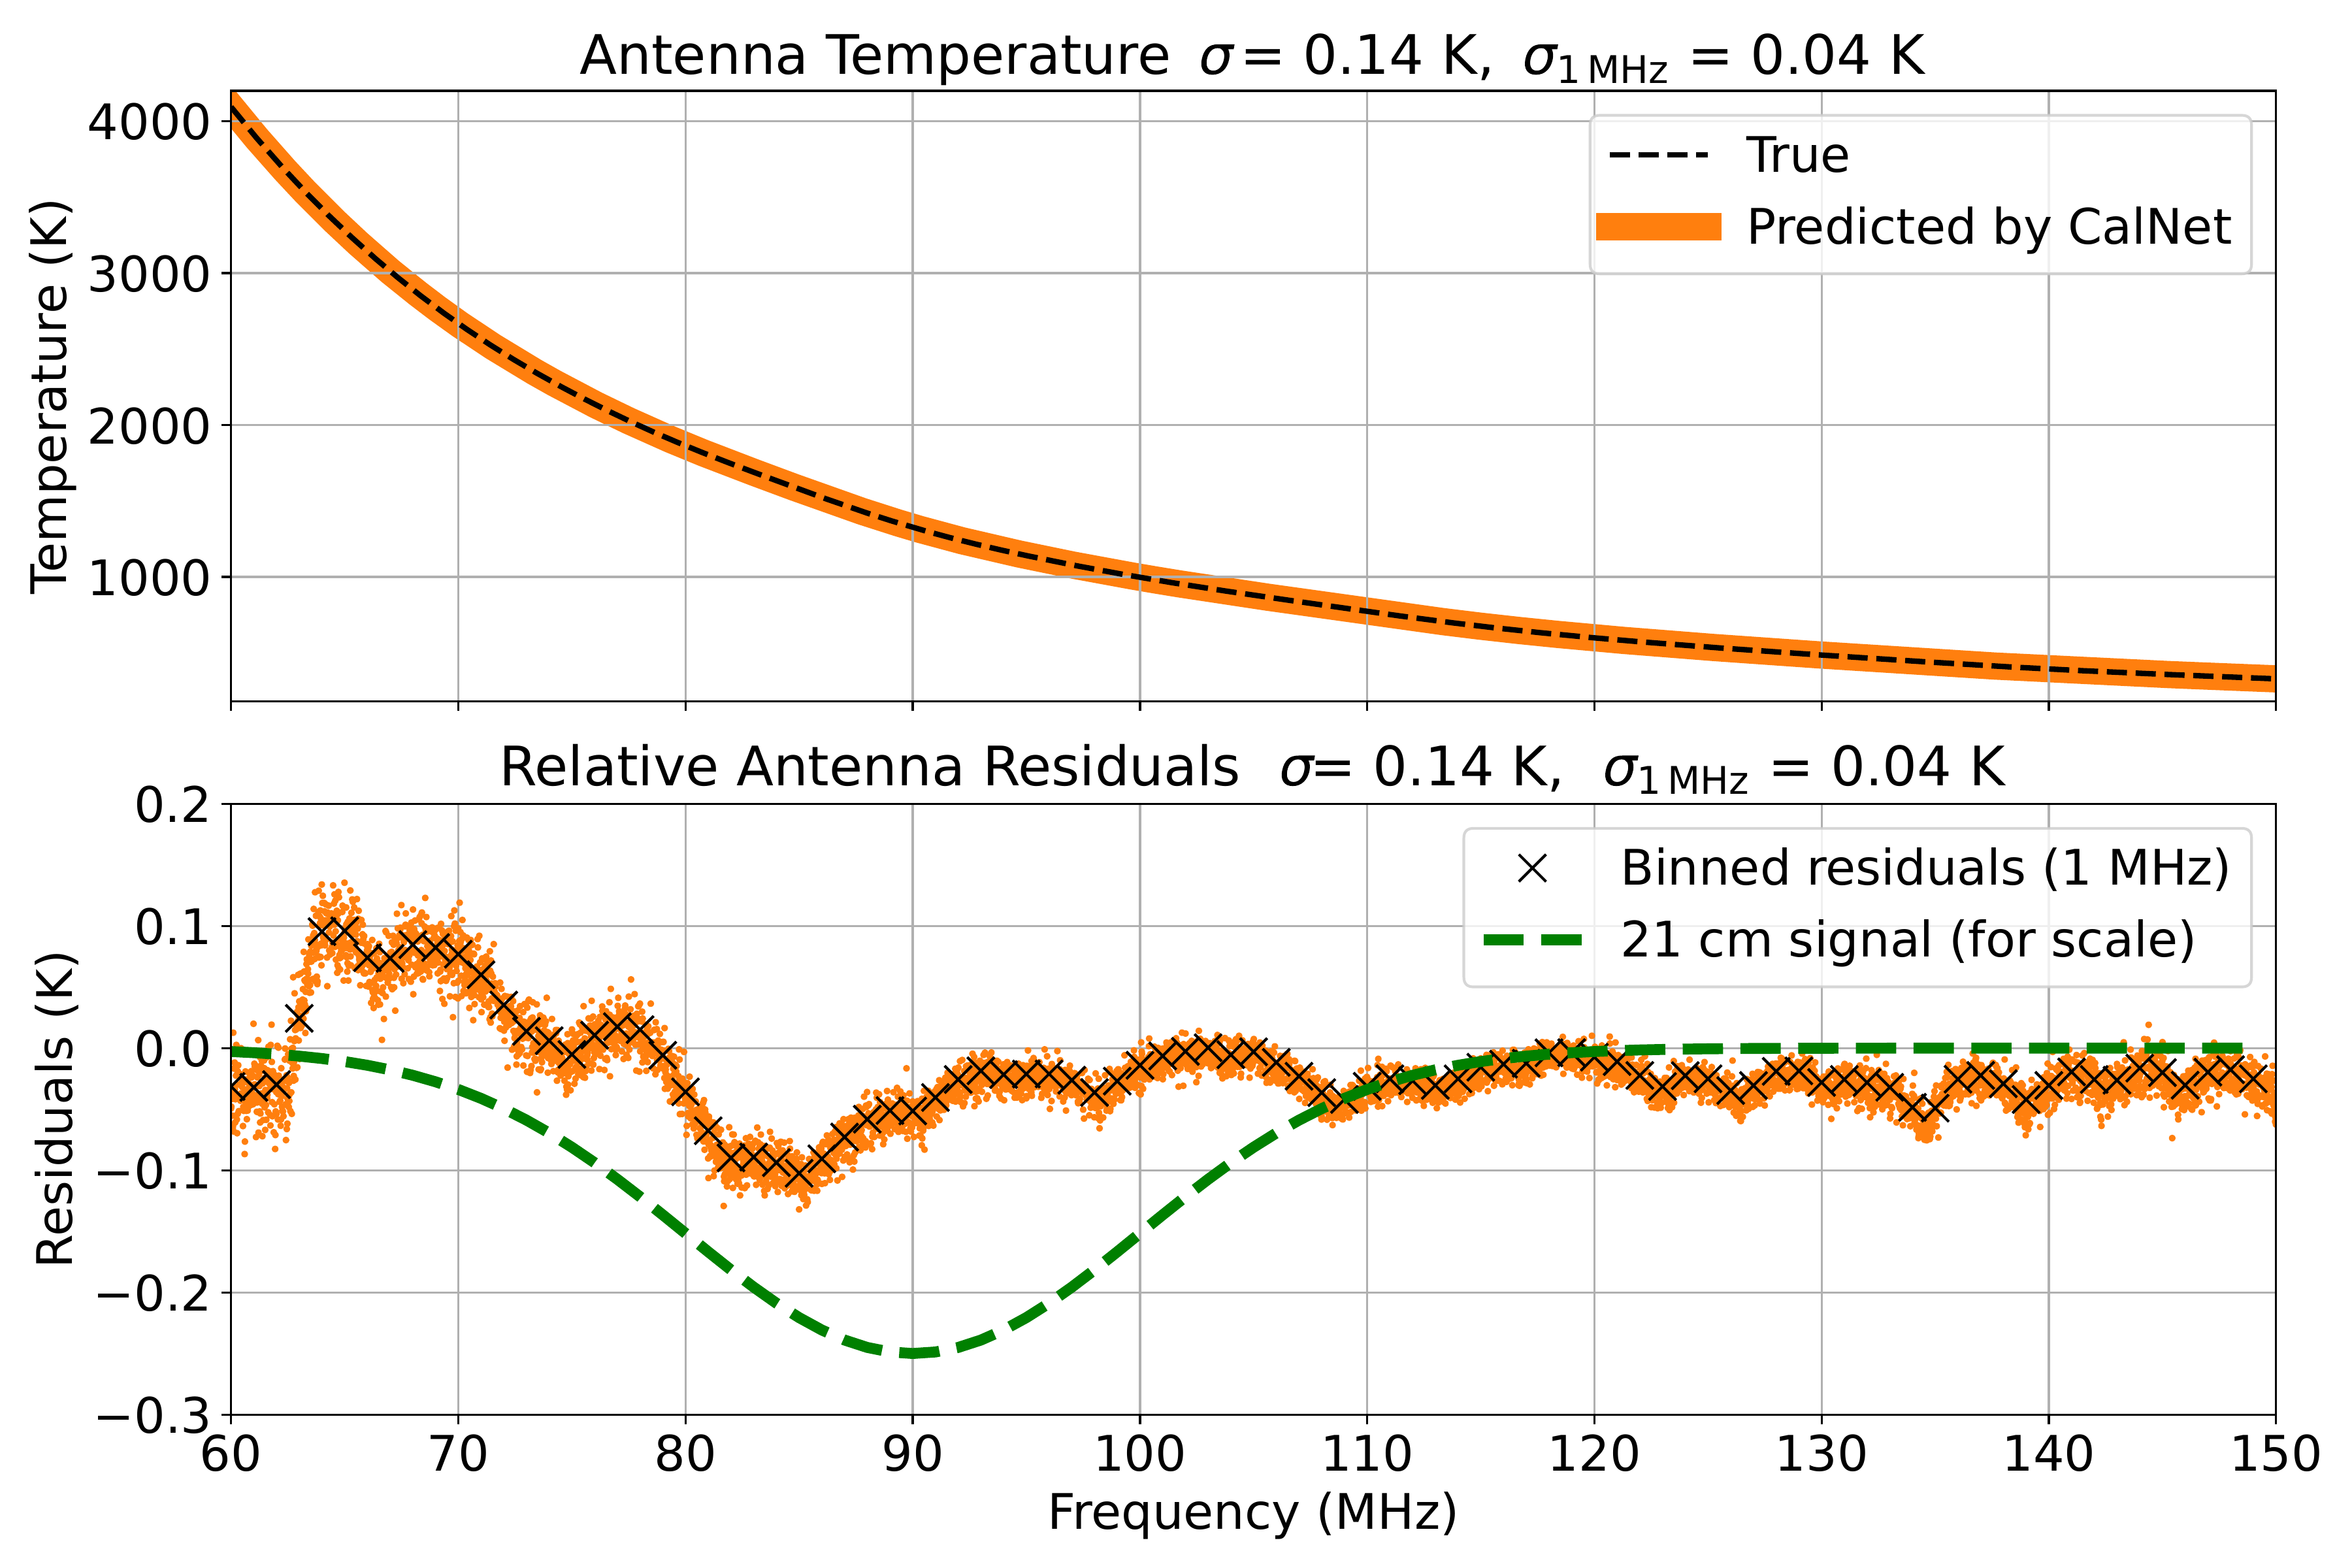
\includegraphics[width=0.6\textwidth]{images/validation_calibrator.pdf}
		\caption{The top panel shows the predicted antenna temperature in orange, with the true temperature overlaid in black dashes}
	\end{figure}
\end{frame}

\begin{frame}{\small{Inferred 21cm Signal}}
	\begin{columns}
		\begin{column}{0.48\textwidth}
			\begin{figure}
				\centering
				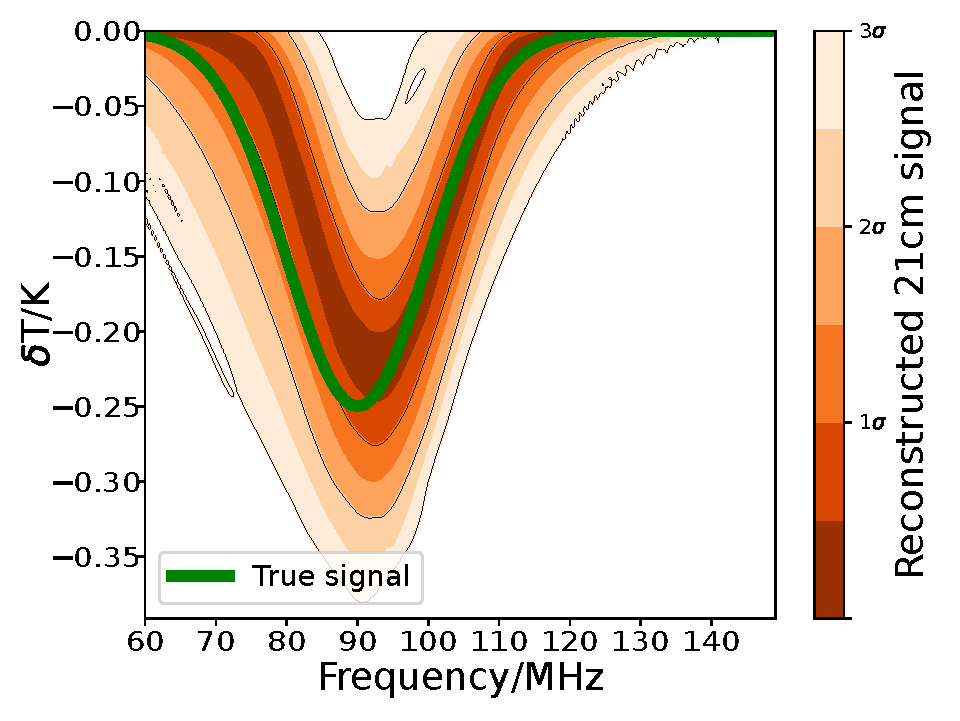
\includegraphics[width=0.9\textwidth]{images/signal_comparison.pdf}
				\caption{\tiny Left: Reconstructed 21cm signal with posterior (orange) and true signal (green)}
			\end{figure}
		\end{column}
		\begin{column}{0.48\textwidth}
			\begin{figure}
				\centering
				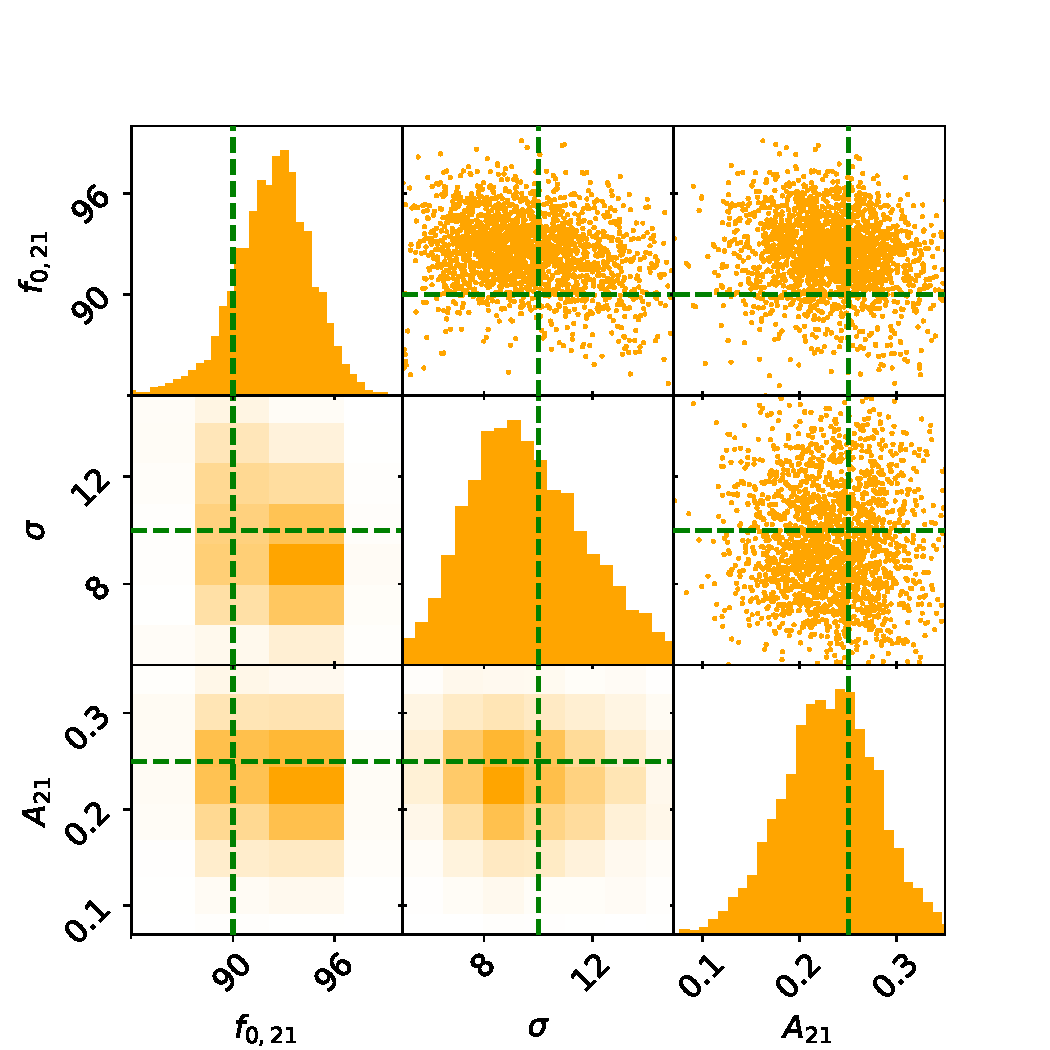
\includegraphics[width=0.9\textwidth]{images/signal_triangle_plot.pdf}
				\caption{\tiny Right: Posterior plots of recovered 21cm signal parameters}
			\end{figure}
		\end{column}
	\end{columns}
\end{frame}

\section{Learning non-linear time-dependent system drift}

\begin{frame}{\small{Neural Network Time Evolution}}
	\begin{figure}
		\centering
		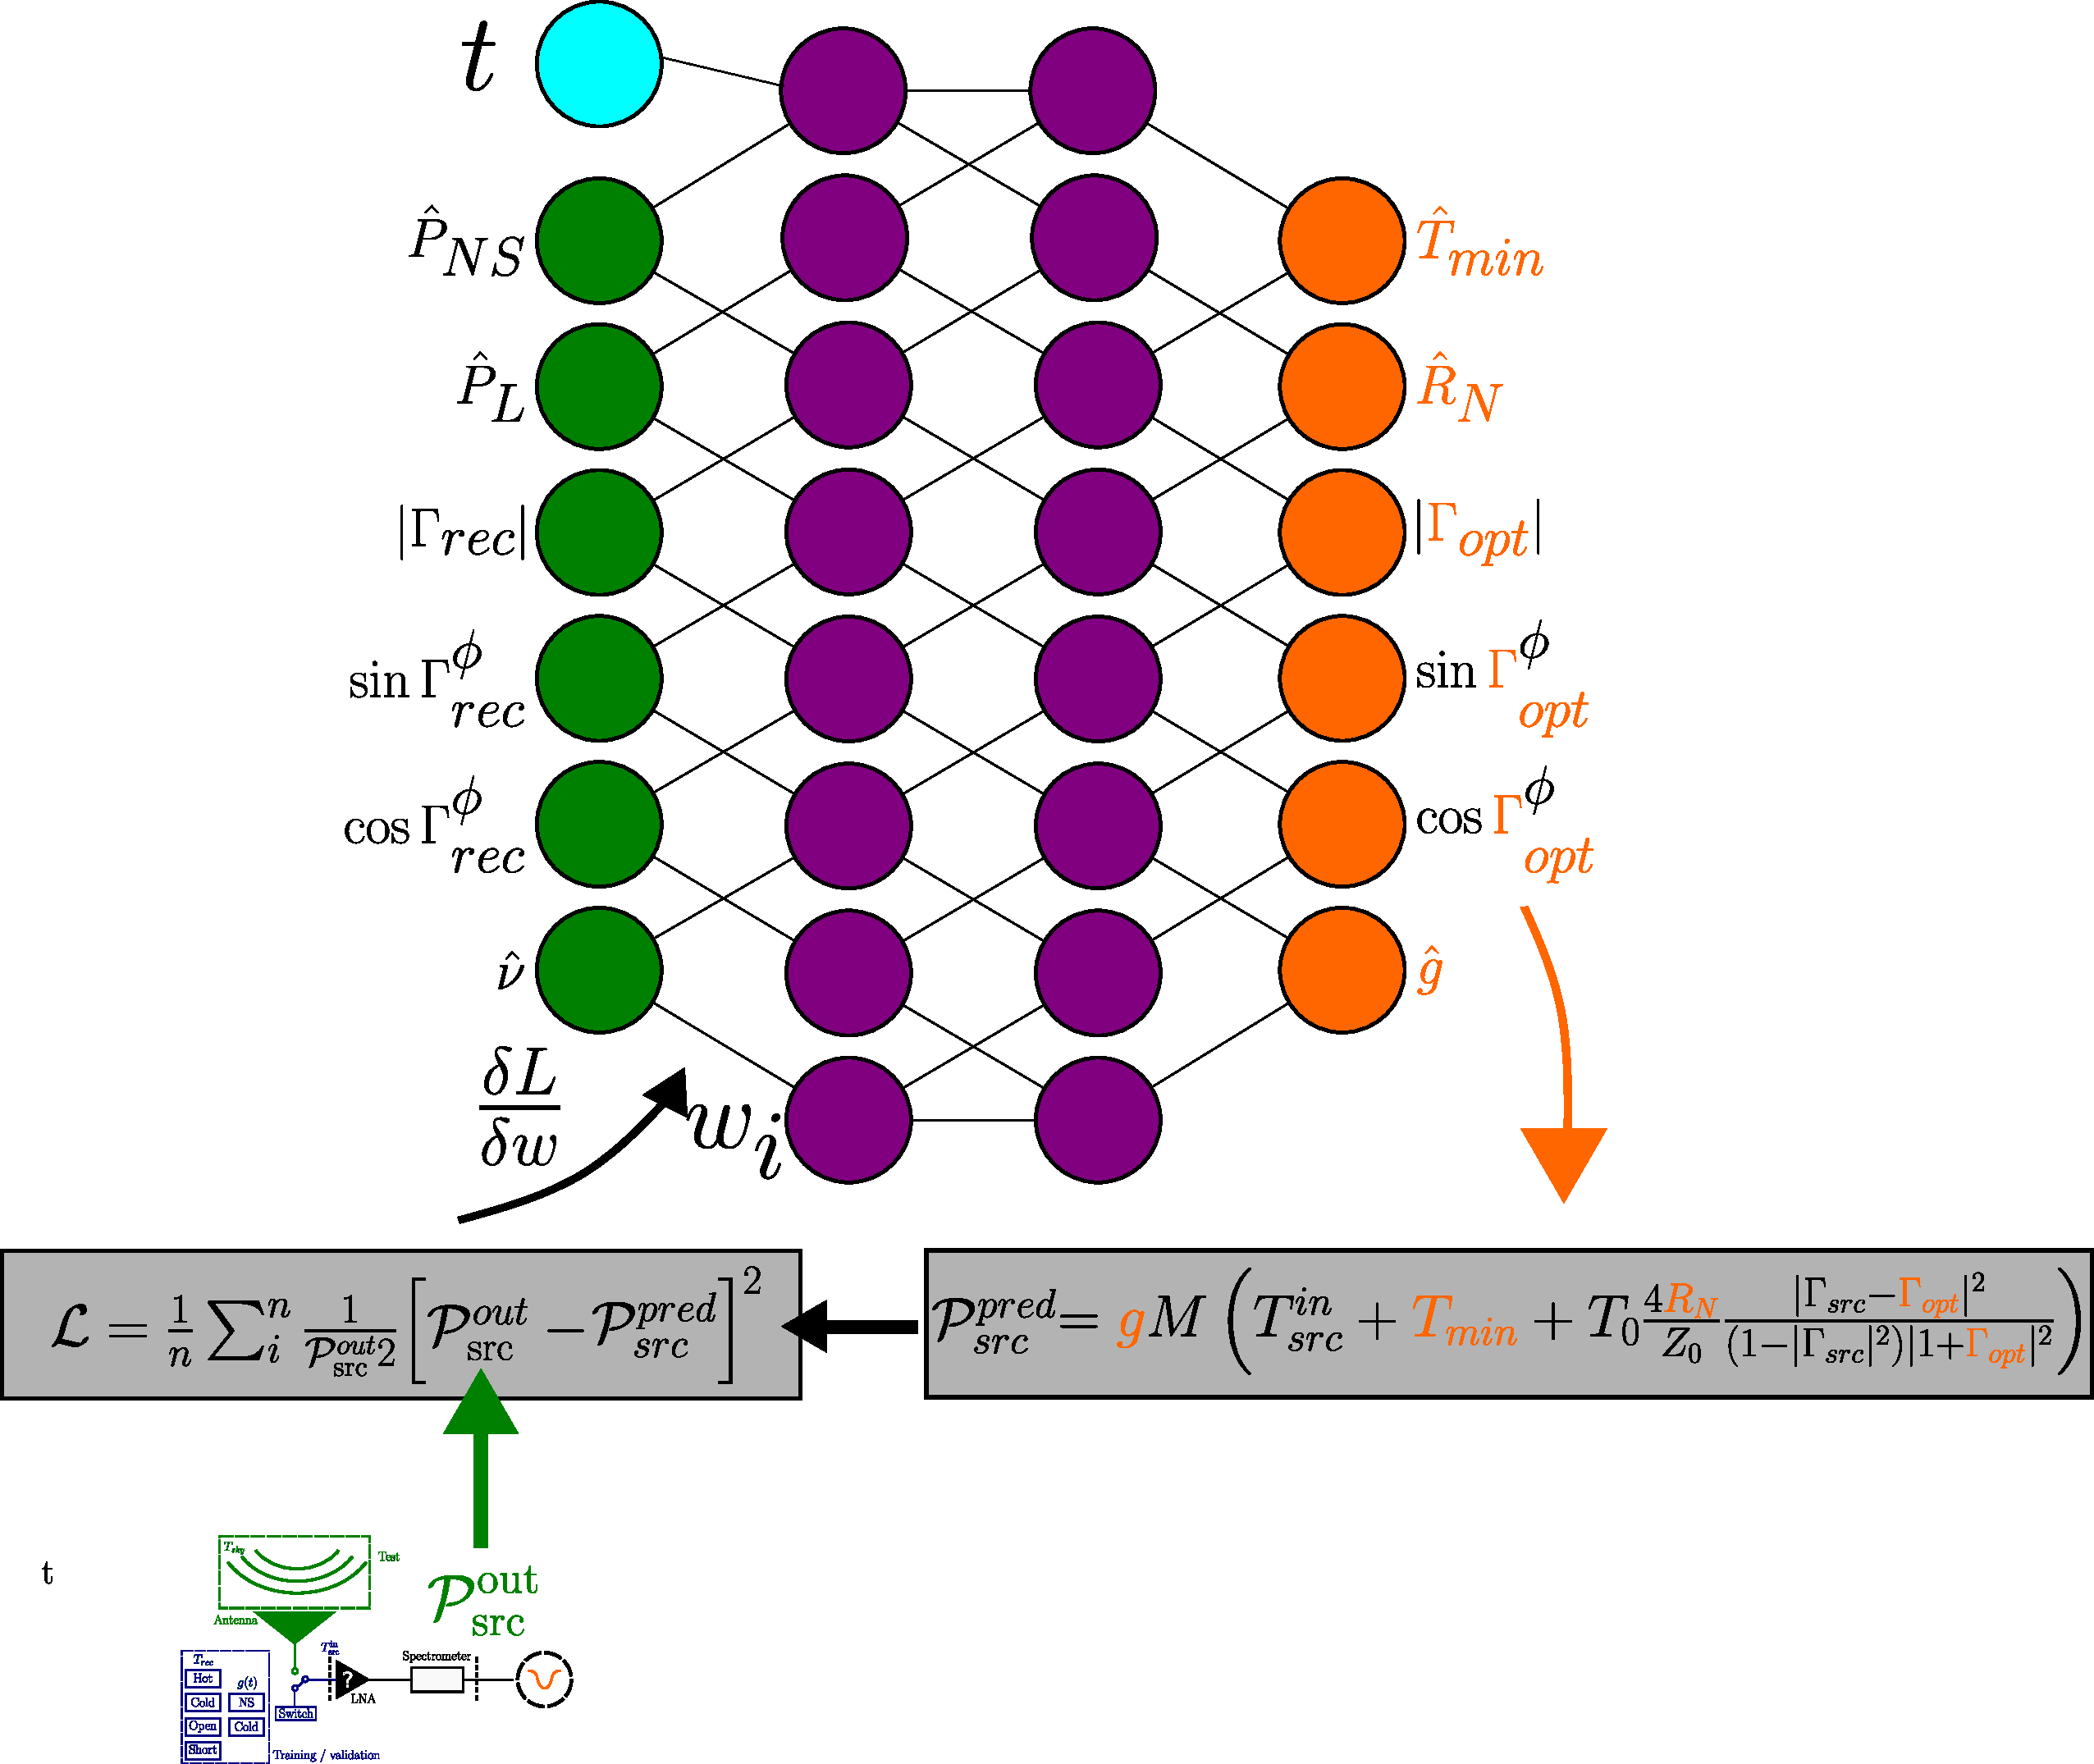
\includegraphics[width=0.5\textwidth]{images/nn_time.pdf}
	\end{figure}
\end{frame}

\begin{frame}{\small{Inject system drift}}
	\centering
	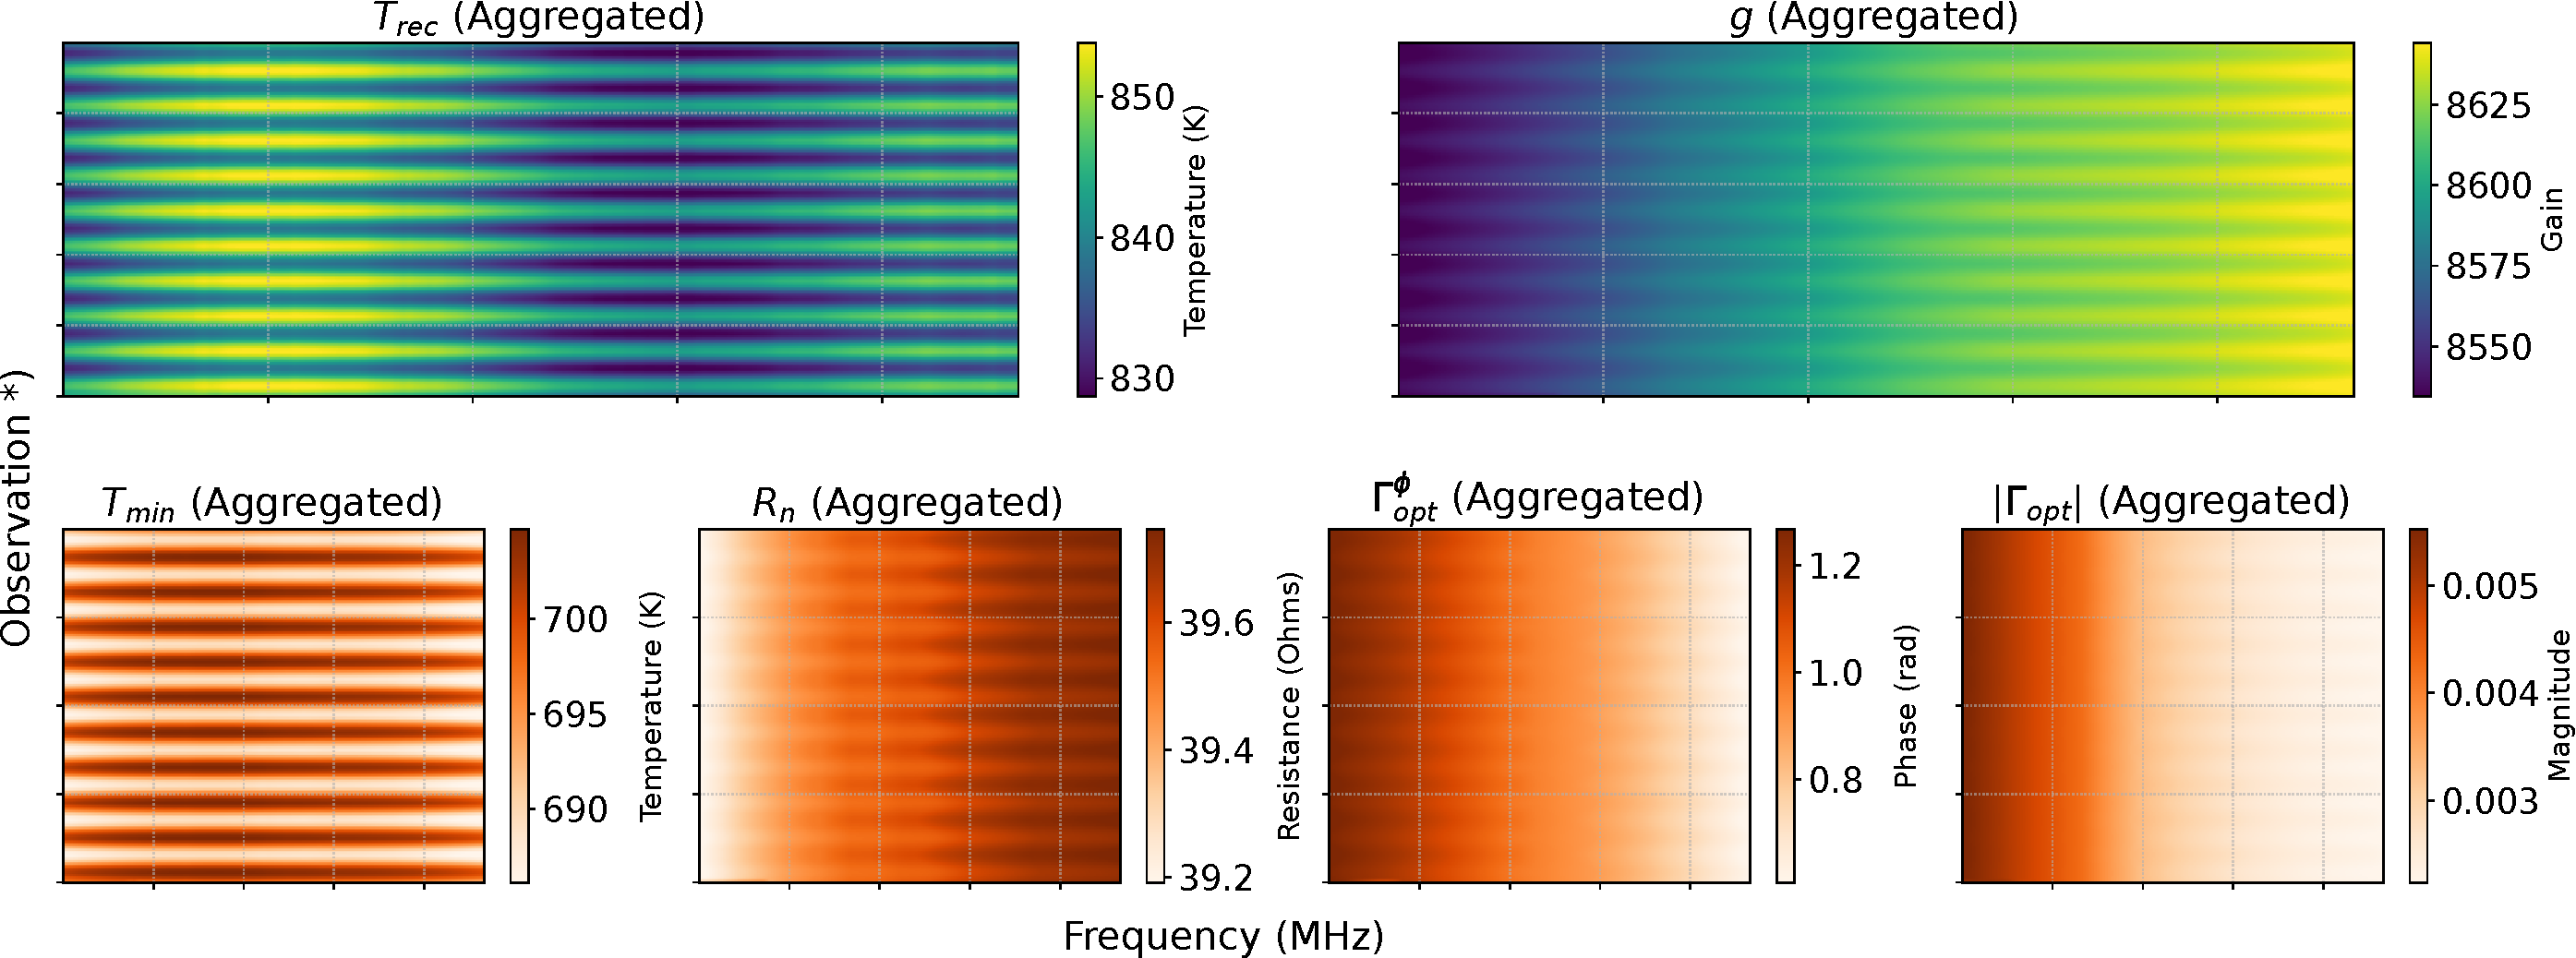
\includegraphics[width=\textwidth]{images/temps_combined_2d.pdf}
	\begin{tcolorbox}[colback=blue!5!white,colframe=blue!75!black,title=]
		Inject a time varying sinusoid into $T_{\text{min}}$ and predict the noise parameters $\rightarrow$ the network recovers this 'system drift'
	\end{tcolorbox}
\end{frame}

\begin{frame}{\small{Single night, many observations}}
	\begin{figure}
		\centering
		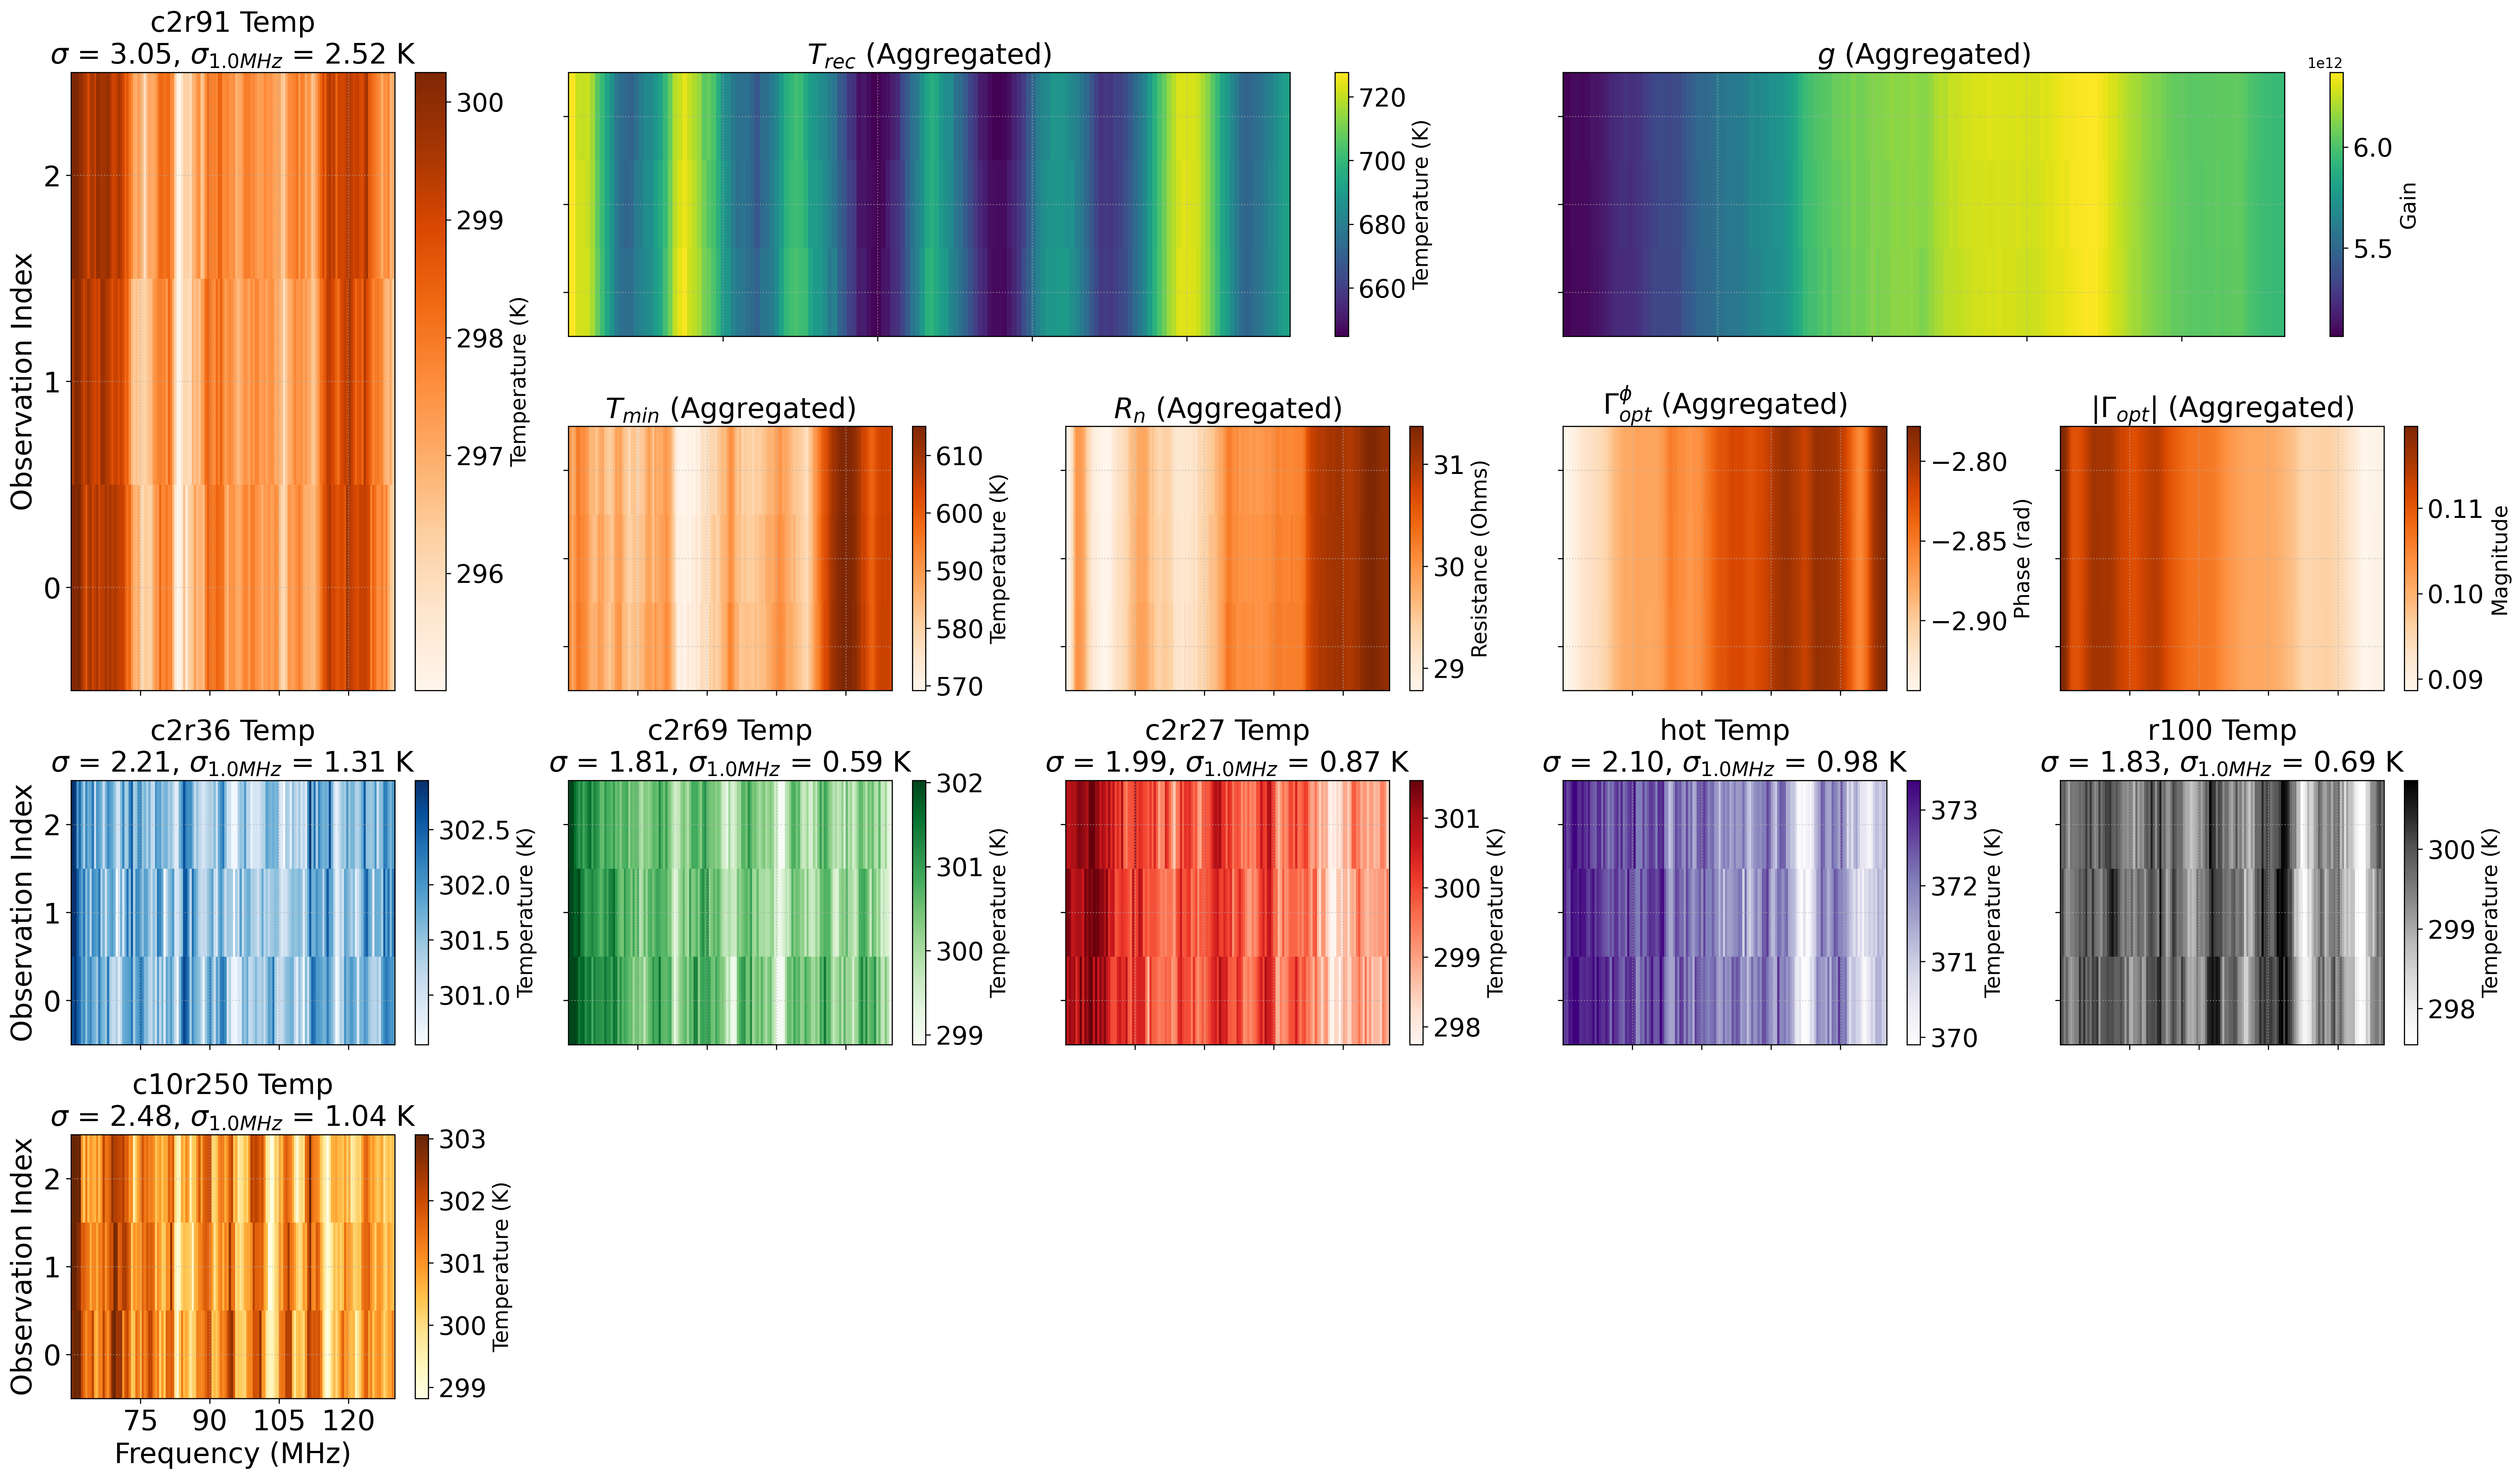
\includegraphics[width=0.8\textwidth]{images/pasted_image_20250403112230.png}
	\end{figure}
\end{frame}

\begin{frame}{\small{Many nights, many observations}}
	\begin{figure}
		\centering
		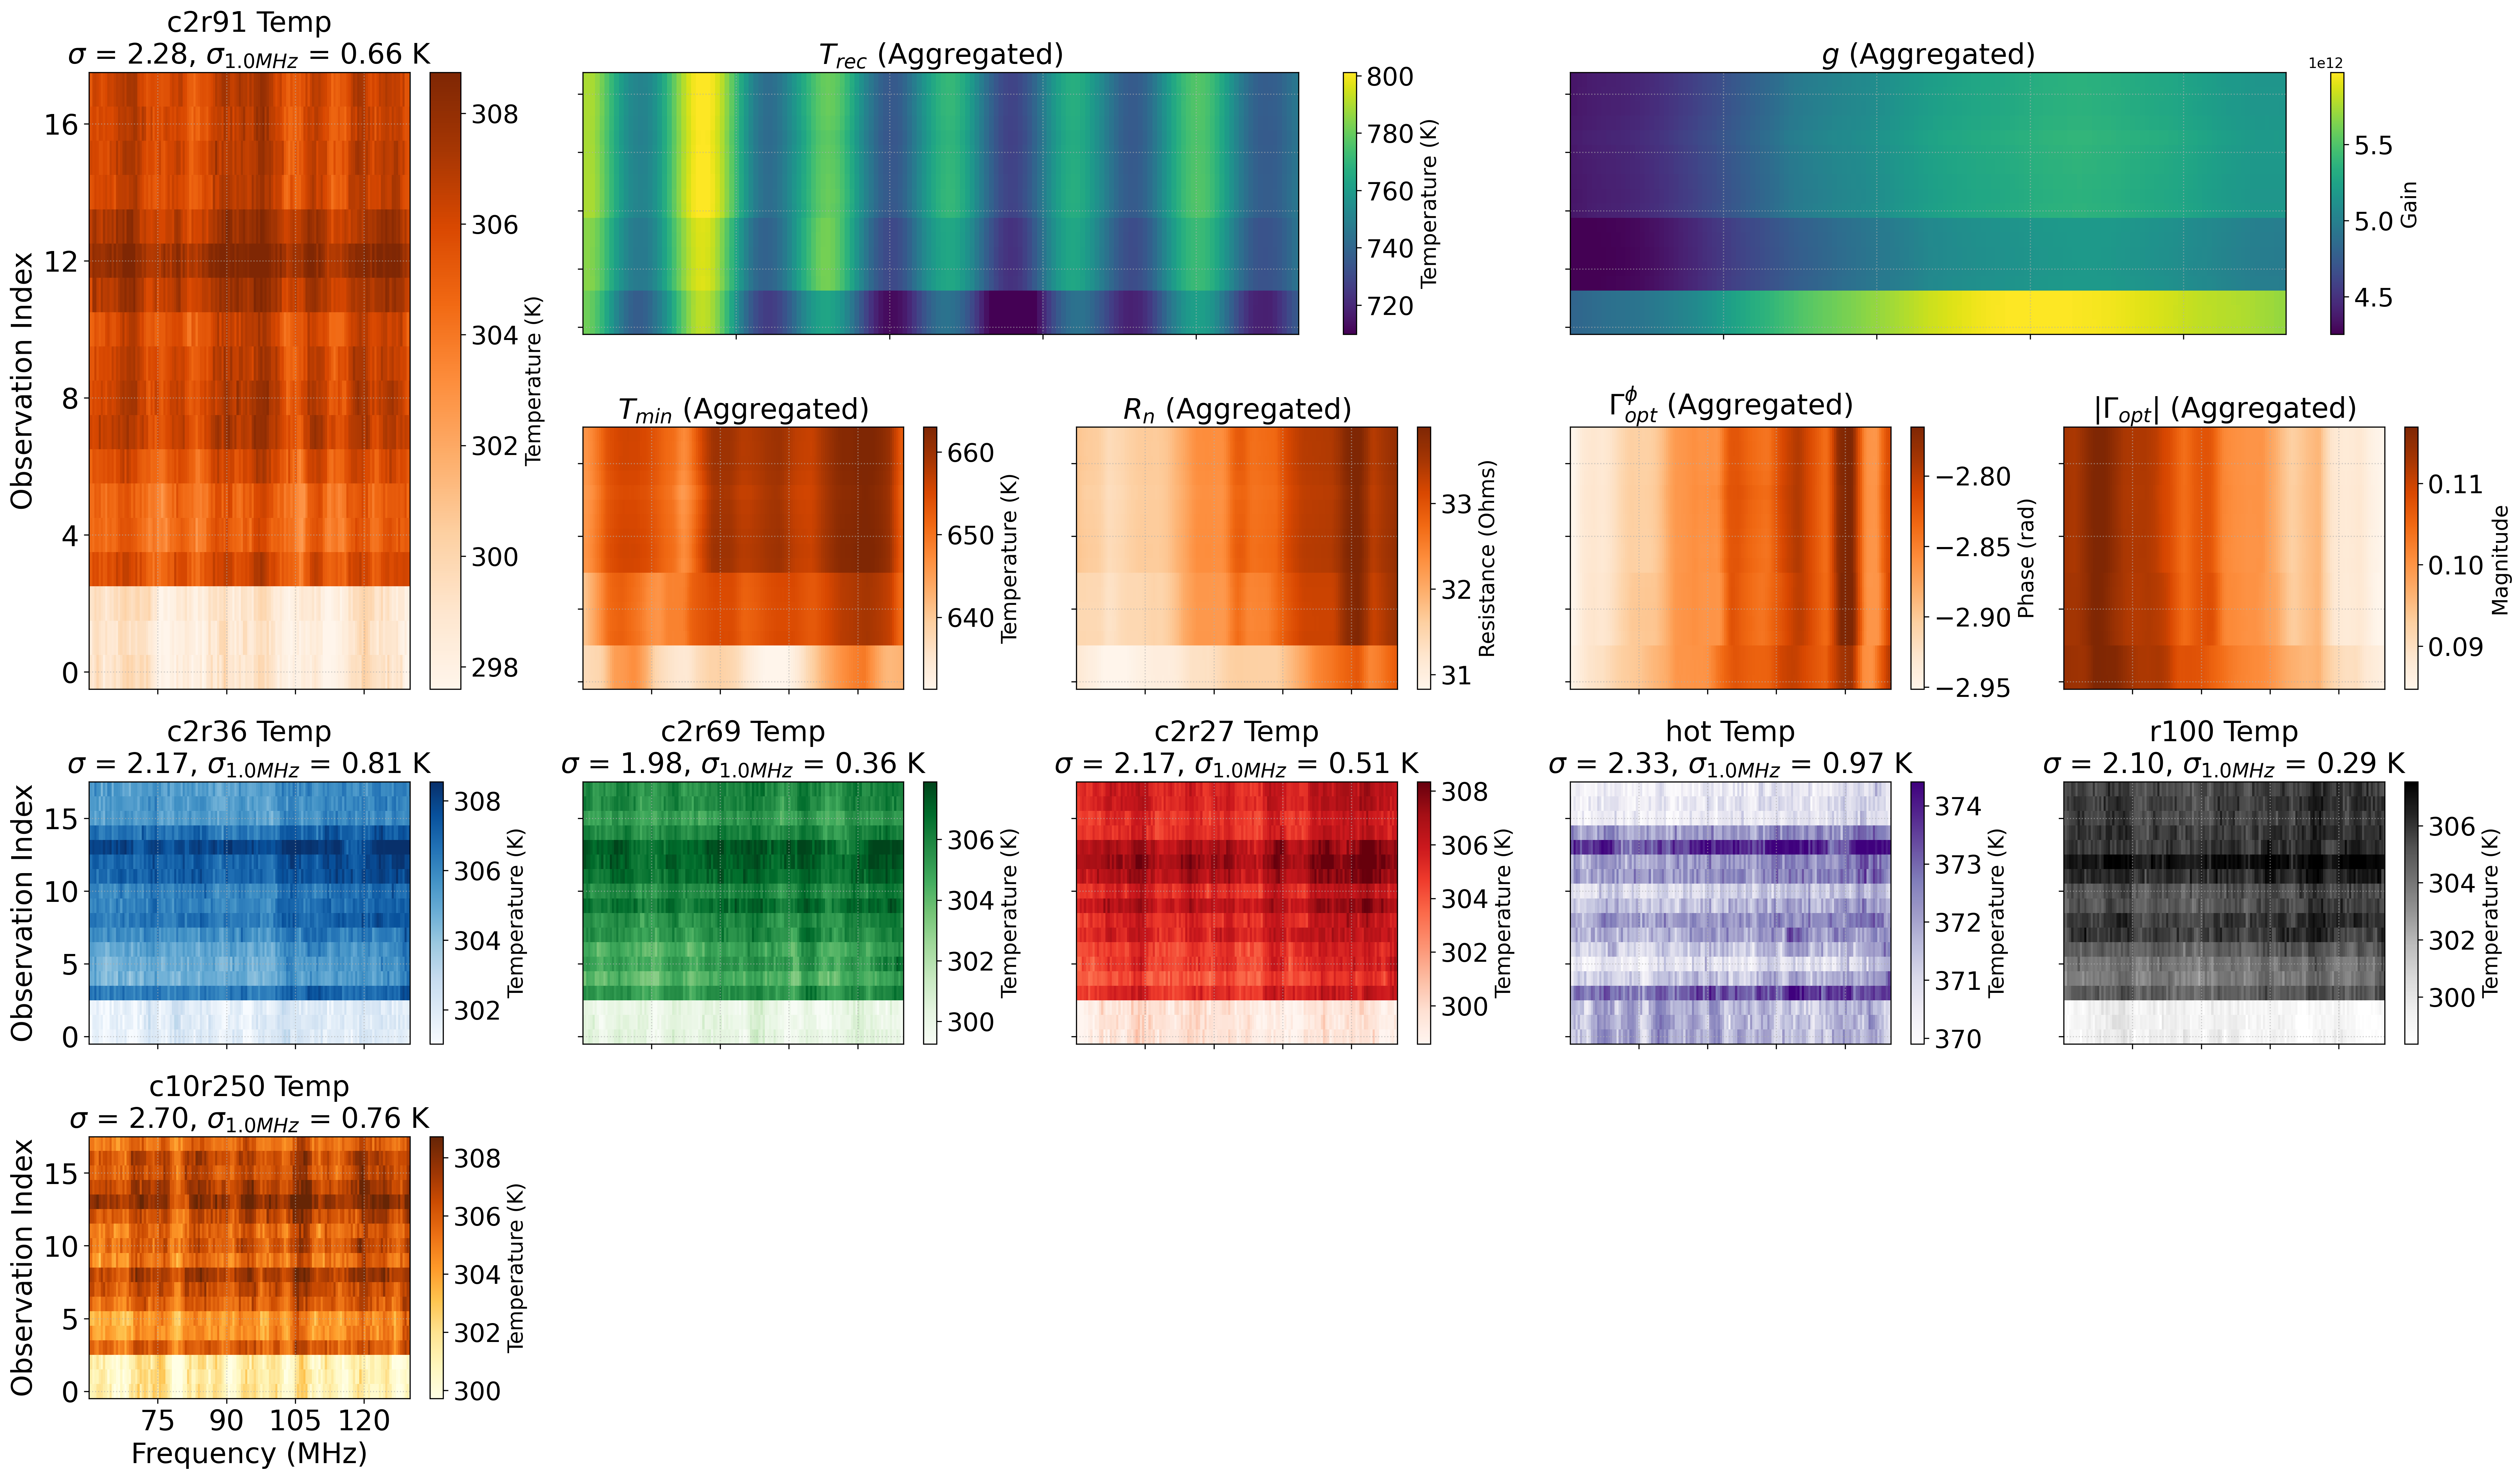
\includegraphics[width=0.8\textwidth]{images/pasted_image_20250410111857.png}
	\end{figure}
\end{frame}

\begin{frame}{\small{Read the paper...}}
	\begin{figure}
		\centering
		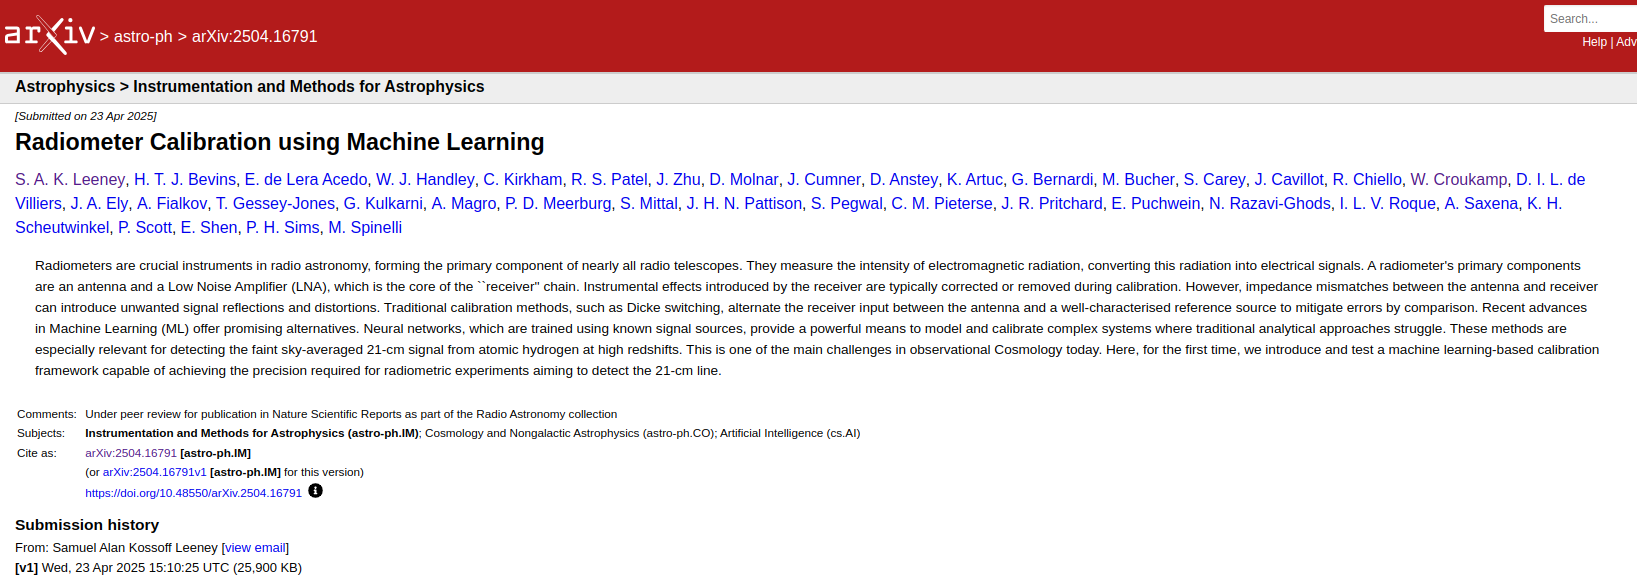
\includegraphics[width=\textwidth]{images/paper_front.png}
	\end{figure}
\end{frame}

\begin{frame}{\small{Calibration Performance}}
	\begin{columns}[c]
		\begin{column}{0.6\textwidth}
			\begin{figure}
				\centering
				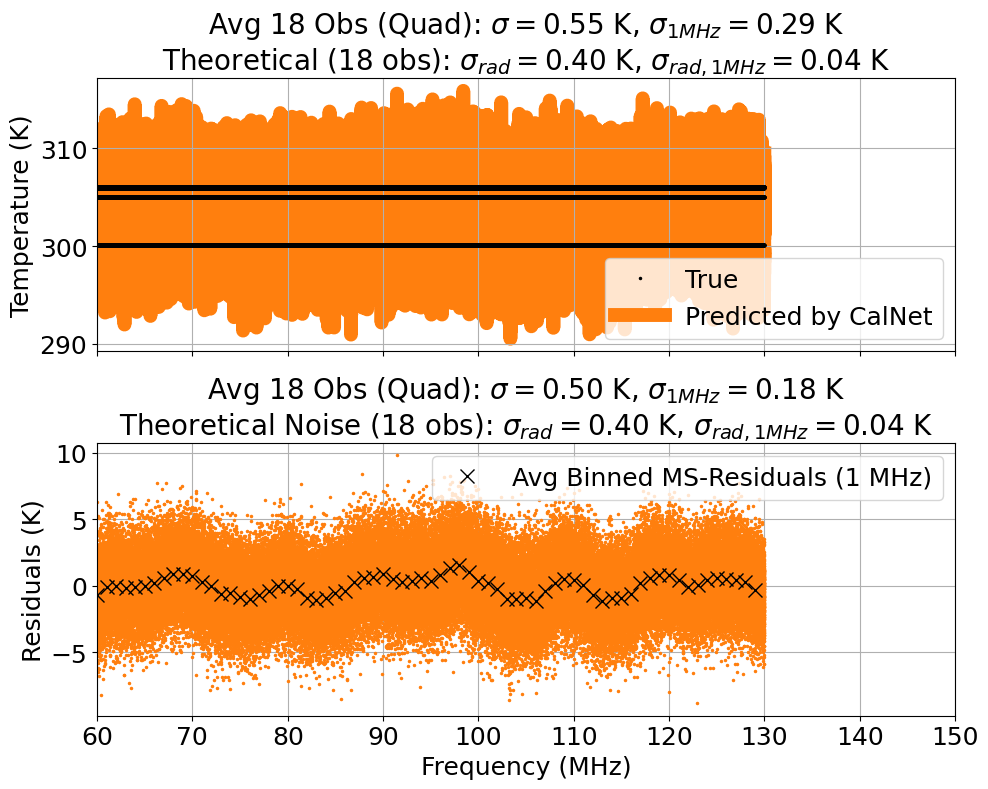
\includegraphics[width=0.9\textwidth]{images/pasted_image_20250515095127.png}
			\end{figure}
		\end{column}
		\begin{column}{0.4\textwidth}
			\begin{itemize}
				\item Significant improvement when combining many nights
				\item Calibration down to 0.18K
				\item Getting close to theoretical noise
			\end{itemize}
		\end{column}
	\end{columns}
\end{frame}

\section{Modeling system drift from other complex system effects}

\begin{frame}{\small{Modeling environmental features}}
	\begin{columns}[c]
		\begin{column}{0.55\textwidth}
			\begin{figure}
				\centering
				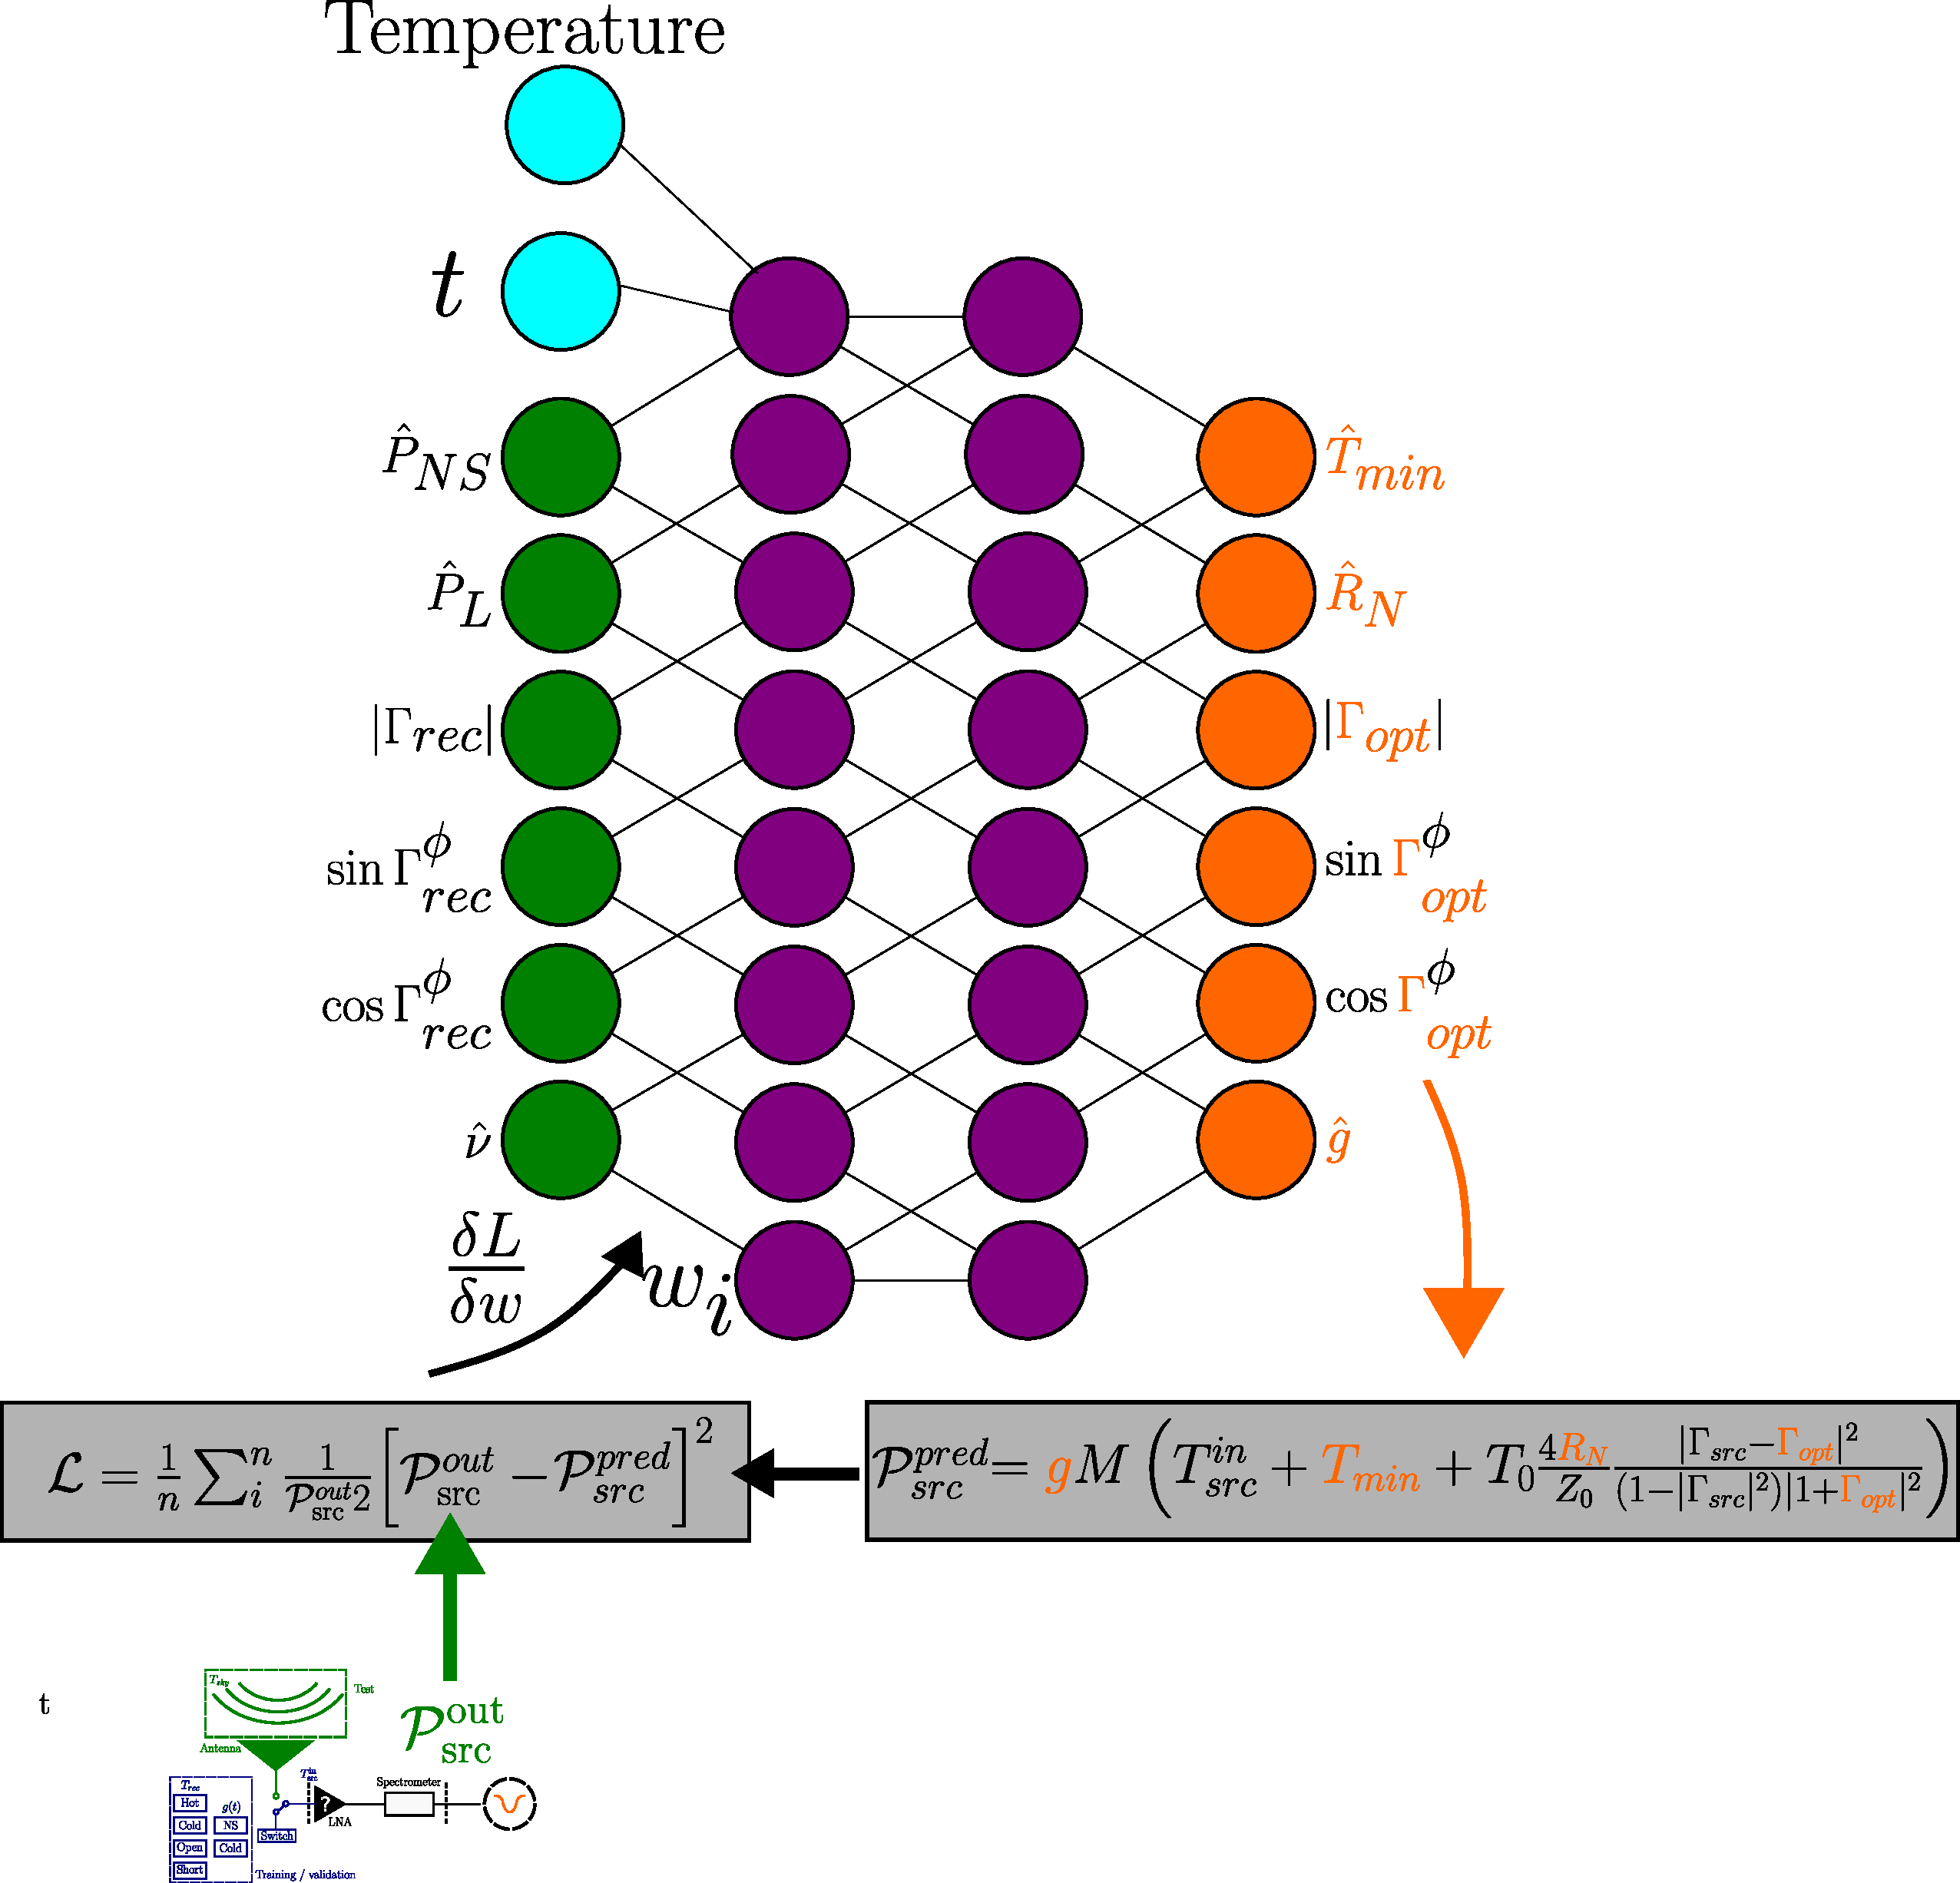
\includegraphics[width=\textwidth]{images/nn_time_tpm.pdf}
				\caption{\tiny Neural network evolution with temperature dependencies}
			\end{figure}
		\end{column}
		\begin{column}{0.45\textwidth}
			\begin{tcolorbox}[colback=blue!5!white,colframe=blue!75!black,title=]
				We can train on features that cannot be modeled analytically
			\end{tcolorbox}
		\end{column}
	\end{columns}
\end{frame}

\begin{frame}{\small{Fitting environmental features against fitted noise parameters}}
	\begin{columns}[c]
		\begin{column}{0.45\textwidth}
			\begin{tcolorbox}[colback=blue!5!white,colframe=blue!75!black,title=]
				Correlate noise parameters with environmental data
			\end{tcolorbox}
		\end{column}
		\begin{column}{0.55\textwidth}
			\begin{figure}
				\centering
				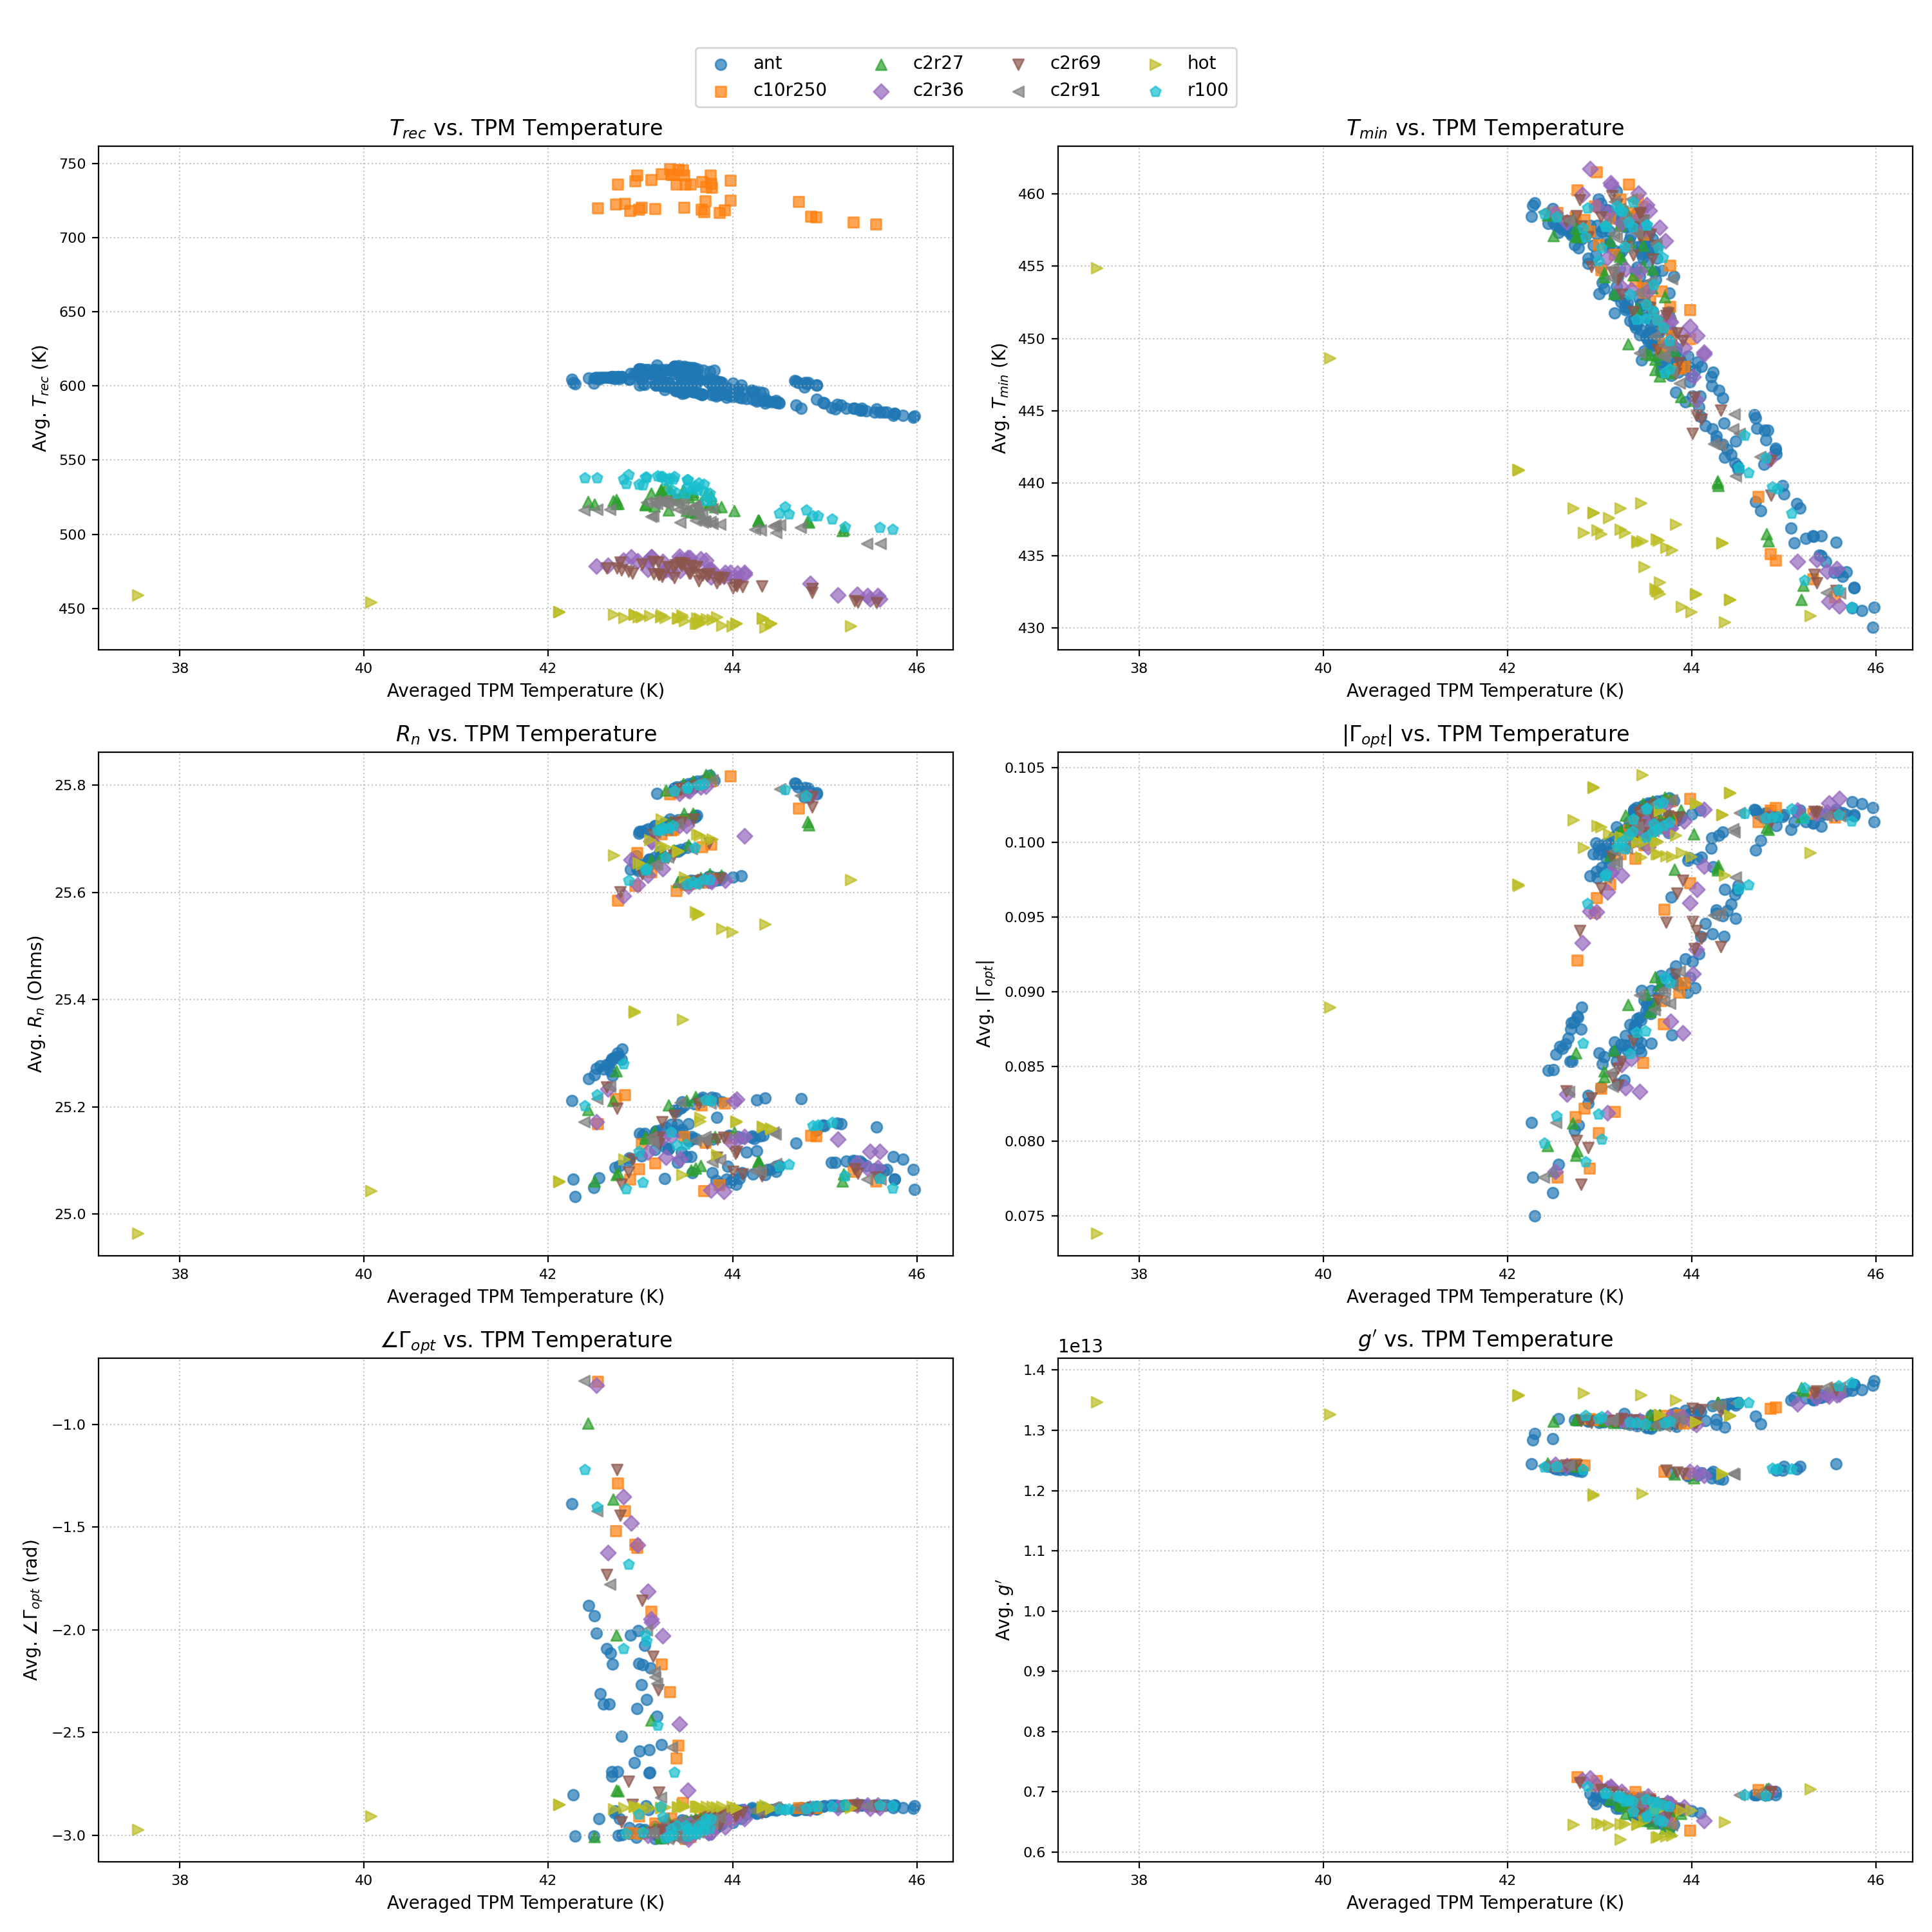
\includegraphics[width=\textwidth]{images/pasted_image_20250605135110.png}
			\end{figure}
		\end{column}
	\end{columns}
\end{frame}

% \begin{frame}{Testing on real data (REACH receiver)}
% 	\begin{figure}
% 		\centering
% 		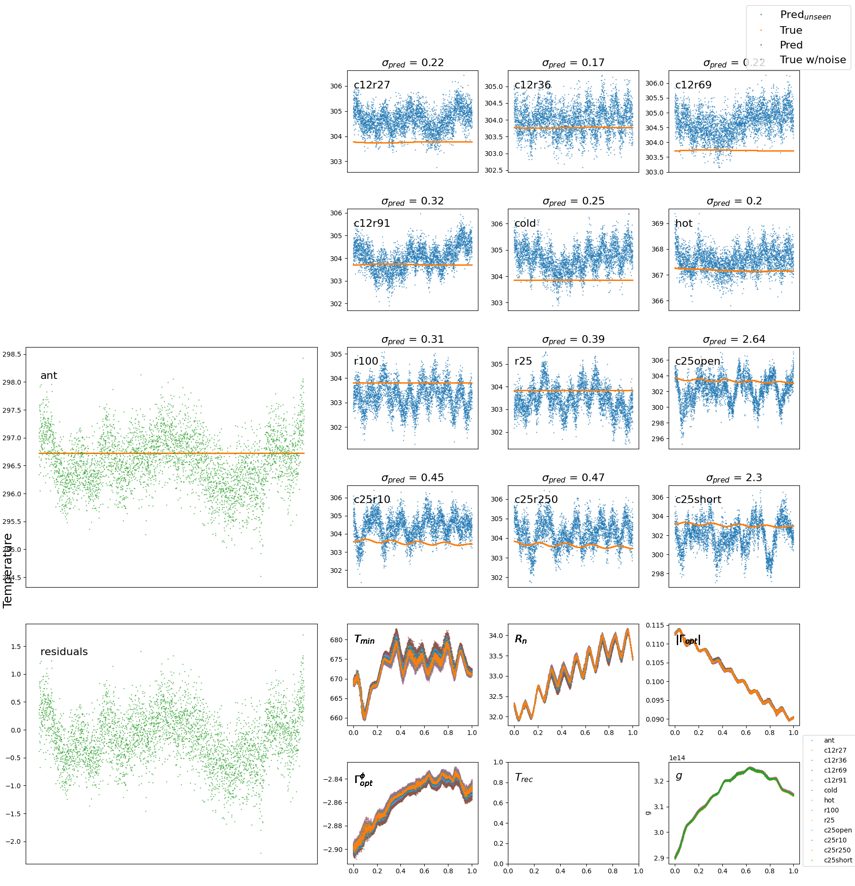
\includegraphics[width=0.5\textwidth]{nima_best.png}
% 	\end{figure}
% \end{frame}

\begin{frame}{\small{Thank you!}}
	\begin{figure}
		\centering
		
\includegraphics[width=0.35\textwidth]{images/qr.png}
	\end{figure}
\end{frame}

\appendix
\section{Appendix}

\begin{frame}{\small{Calibration Equation}}

	\vspace{0.2cm} % Adds a small vertical space at the top

	\textbf{Typically, substitute in the noise wave parameter equation here (gains cancel)}

	\vspace{0.2cm} % Adds space between text and first equation

	% Calibration Equation with \tiny font and manual tag (4)
	{\tiny
		\begin{equation}
			T_{\text{cal}}^* = T_{\text{NS}} \frac{P_{\text{cal}} - P_L}{P_{\text{NS}} - P_L} + T_L \tag{4}
		\end{equation}
	}

	\vspace{0.1cm} % Adds space between equation and next text

	\textbf{Make some matching assumptions and re arrange:}

	\vspace{0.1cm} % Adds space between text and second equation

	% Multline Equation with \tiny font and manual tag (5)
	{\tiny
		\begin{multline}
			T_\mathrm{s} = \textcolor{red}{T_\mathrm{NS}}\left(\frac{P_\mathrm{s} - P_\mathrm{L}}{P_\mathrm{NS} - P_\mathrm{L}}\right)\frac{\left|1 - \Gamma_\mathrm{s}\Gamma_\mathrm{rec}\right|^2}{1 - |\Gamma_\mathrm{s}|^2} + \textcolor{red}{T_\mathrm{L}}\frac{\left|1 - \Gamma_\mathrm{s}\Gamma_\mathrm{rec}\right|^2}{1 - |\Gamma_\mathrm{s}|^2} - \textcolor{red}{T_\mathrm{unc}} \frac{|\Gamma_\mathrm{s}|^2}{1 - |\Gamma_\mathrm{s}|^2} +  \\
			-\textcolor{red}{T_\mathrm{cos}} \frac{\Re \left( \frac{\Gamma_\mathrm{s}}{1 - \Gamma_\mathrm{s}\Gamma_\mathrm{rec}} \right)\left|1 - \Gamma_\mathrm{s}\Gamma_\mathrm{rec}\right|^2}{(1 - |\Gamma_\mathrm{s}|^2) \sqrt{1 - |\Gamma_\mathrm{rec}|^2}}  -\textcolor{red}{T_\mathrm{sin}} \frac{\Im \left( \frac{\Gamma_\mathrm{s}}{1 - \Gamma_\mathrm{s}\Gamma_\mathrm{rec}} \right)\left|1 - \Gamma_\mathrm{s}\Gamma_\mathrm{rec}\right|^2}{(1 - |\Gamma_\mathrm{s}|^2) \sqrt{1 - |\Gamma_\mathrm{rec}|^2}} \tag{5}
		\end{multline}
	}

	\textit{Note: We end up with 5 parameters that need to be estimated to calibrate the system.}

	\vfill % Pushes the note to the bottom
\end{frame}

\begin{frame}{\small{Calculating the error}}

	% Adding a block
	\textbf{By partial derivatives}
	To find the error in \( T_s \), we propagate the errors in \( \Gamma_s \), \( \Gamma_{rec} \), \( P_L \), \( P_{NS} \), and \( P_s \):
	%
	\begin{multline}
		(\Delta T_s)^2 = \left(\frac{\partial T_s}{\partial \Gamma_s} \Delta \Gamma_s\right)^2 + \left(\frac{\partial T_s}{\partial \Gamma_{rec}} \Delta \Gamma_{rec}\right)^2 \\ + \left(\frac{\partial T_s}{\partial P_L} \Delta P_L\right)^2 + \left(\frac{\partial T_s}{\partial P_{NS}} \Delta P_{NS}\right)^2 + \left(\frac{\partial T_s}{\partial P_s} \Delta P_s\right)^2.
	\end{multline}
	%

\end{frame}

\begin{frame}{\small{Calculating the error}}
	\vfill
	{\tiny
		\begin{multline}
			(\Delta T_s)^2 =
			\left(\frac{\partial T_s}{\partial \Gamma_s} \Delta \Gamma_s\right)^2 +
			\left(\frac{\partial T_s}{\partial \Gamma_{rec}} \Delta \Gamma_{rec}\right)^2 +
			\left(\frac{\partial T_s}{\partial P_L} \Delta P_L\right)^2 +
			\left(\frac{\partial T_s}{\partial P_{NS}} \Delta P_{NS}\right)^2 +
			\left(\frac{\partial T_s}{\partial P_s} \Delta P_s\right)^2.
		\end{multline}
	}

	\hrule

	\begin{columns}[c] % Align columns centrally inside the box
		\begin{column}{0.4\textwidth}
			\centering
			{\tiny
				\begin{align}
					\frac{\partial T_s}{\partial P_L}    & = T_\mathrm{NS} \frac{\left|1 - \Gamma_\mathrm{s} \Gamma_\mathrm{rec}\right|^2}{1 - |\Gamma_\mathrm{s}|^2} \cdot \frac{P_\mathrm{s} - P_\mathrm{NS}}{(P_\mathrm{NS} - P_\mathrm{L})^2}, \\
					\frac{\partial T_s}{\partial P_{NS}} & = -T_\mathrm{NS} \frac{\left|1 - \Gamma_\mathrm{s} \Gamma_\mathrm{rec}\right|^2}{1 - |\Gamma_\mathrm{s}|^2} \cdot \frac{P_\mathrm{s} - P_\mathrm{L}}{(P_\mathrm{NS} - P_\mathrm{L})^2}, \\
					\frac{\partial T_s}{\partial P_s}    & = T_\mathrm{NS} \left(\frac{1}{P_\mathrm{NS}-P_\mathrm{L}}\right) \frac{\left|1-\Gamma_\mathrm{s}\Gamma_\mathrm{rec}\right|^2}{ 1-|\Gamma_\mathrm{s}|^2}.
				\end{align}

				\begin{equation}
					\frac{\partial T_s}{\partial \Gamma_{rec}} = \frac{\partial A}{\partial \Gamma_{rec}} + \frac{\partial B}{\partial \Gamma_{rec}} + \frac{\partial D}{\partial \Gamma_{rec}} + \frac{\partial E}{\partial \Gamma_{rec}}.
				\end{equation}

				\begin{equation}
					\frac{\partial T_s}{\partial \Gamma_s} = \frac{\partial A}{\partial \Gamma_s} + \frac{\partial B}{\partial \Gamma_s} + \frac{\partial C}{\partial \Gamma_s} + \frac{\partial D}{\partial \Gamma_s} + \frac{\partial E}{\partial \Gamma_s}.
				\end{equation}
			}
		\end{column}

		\begin{column}{0.6\textwidth}
			{\tiny
				\begin{align}
					A & = T_\mathrm{NS}\left(\frac{P_\mathrm{s} - P_\mathrm{L}}{P_\mathrm{NS}-P_\mathrm{L}}\right)\frac{\left|1-\Gamma_\mathrm{s}\Gamma_\mathrm{rec}\right|^2}{ 1-|\Gamma_\mathrm{s}|^2},                                               \\
					B & = T_\mathrm{L}\frac{\left|1-\Gamma_\mathrm{s}\Gamma_\mathrm{rec}\right|^2}{ 1-|\Gamma_\mathrm{s}|^2},                                                                                                                           \\
					C & = - T_\mathrm{unc} \frac{ |\Gamma_\mathrm{s}|^2}{1-\left|\Gamma_\mathrm{s}\right|^2},                                                                                                                                           \\
					D & = -T_\mathrm{cos} \frac{\Re \left( \frac{ \Gamma_\mathrm{s}}{1-\Gamma_\mathrm{s}\Gamma_\mathrm{rec}}\right)\left|1-\Gamma_\mathrm{s}\Gamma_\mathrm{rec}\right|^2}{( 1-|\Gamma_\mathrm{s}|^2) \sqrt{1-|\Gamma_\mathrm{rec}|^2}}, \\
					E & = -T_\mathrm{sin} \frac{\Im \left( \frac{ \Gamma_\mathrm{s}}{1-\Gamma_\mathrm{s}\Gamma_\mathrm{rec}}\right)\left|1-\Gamma_\mathrm{s}\Gamma_\mathrm{rec}\right|^2}{( 1-|\Gamma_\mathrm{s}|^2) \sqrt{1-|\Gamma_\mathrm{rec}|^2}}.
				\end{align}
			}
		\end{column}
	\end{columns}
\end{frame}

\begin{frame}{\small{Calculating the error}}

	% Adding a block
	\textbf{Using $T_{\text{NS}} \frac{P_{\text{cal}} - P_L}{P_{\text{NS}} - P_L} + T_L$}
	%
	\begin{align}
		(\Delta T_s)^2 & = \left(\frac{\partial T_s}{\partial P_s} \Delta P_s\right)^2 + \left(\frac{\partial T_s}{\partial P_L} \Delta P_L\right)^2 + \left(\frac{\partial T_s}{\partial P_{NS}} \Delta P_{NS}\right)^2 \\ &+ \left(\frac{\partial T_s}{\partial \Gamma_s} \Delta \Gamma_s\right)^2 + \left(\frac{\partial T_s}{\partial \Gamma_{rec}} \Delta \Gamma_{rec}\right)^2.
	\end{align}
	%

	\hrule
	\textbf{Using noise wave parameters \textit{only}}
	%
	\begin{align}
		(\Delta T_\mathrm{s})^2 & = \left(\frac{\partial T_\mathrm{s}}{\partial P_\mathrm{s}} \Delta P_\mathrm{s}\right)^2 \\ &+ \left(\frac{\partial T_\mathrm{s}}{\partial \Gamma_\mathrm{s}} \Delta \Gamma_\mathrm{s}\right)^2 + \left(\frac{\partial T_\mathrm{s}}{\partial \Gamma_\mathrm{rec}} \Delta \Gamma_\mathrm{rec}\right)^2.
	\end{align}
	%
	\textit{Note that this argument applies for both noise parameters and noise wave parameters.}

\end{frame}

\begin{frame}

	\begin{columns}
		\begin{column}{0.2\textwidth}
			There is more noise when using $T_{\text{NS}} \frac{P_{\text{cal}} - P_L}{P_{\text{NS}} - P_L} + T_L$
		\end{column}
		\begin{column}{0.8\textwidth}
			\begin{figure}[h]
				\centering
				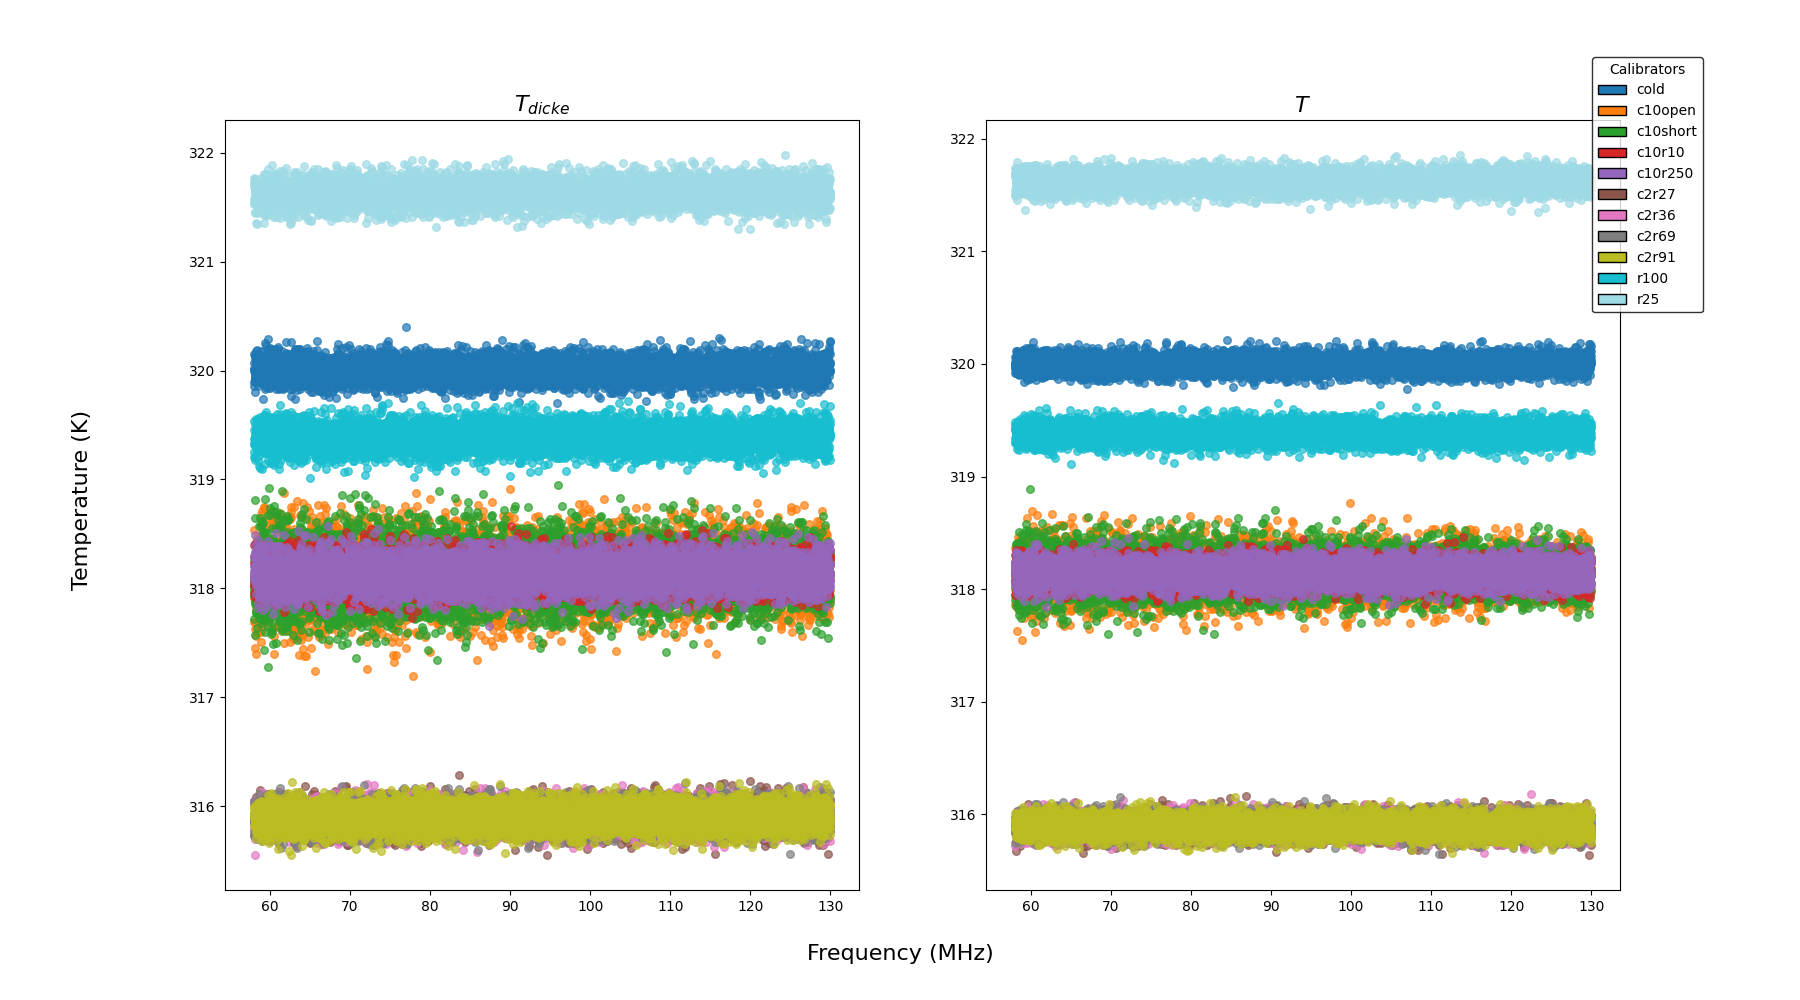
\includegraphics[width=1\textwidth]{images/main_scatter_plots.png}
			\end{figure}
		\end{column}
	\end{columns}

\end{frame}


\begin{frame}
	\begin{columns}
		\begin{column}{0.8\textwidth}
			\begin{figure}[h]
				\centering
				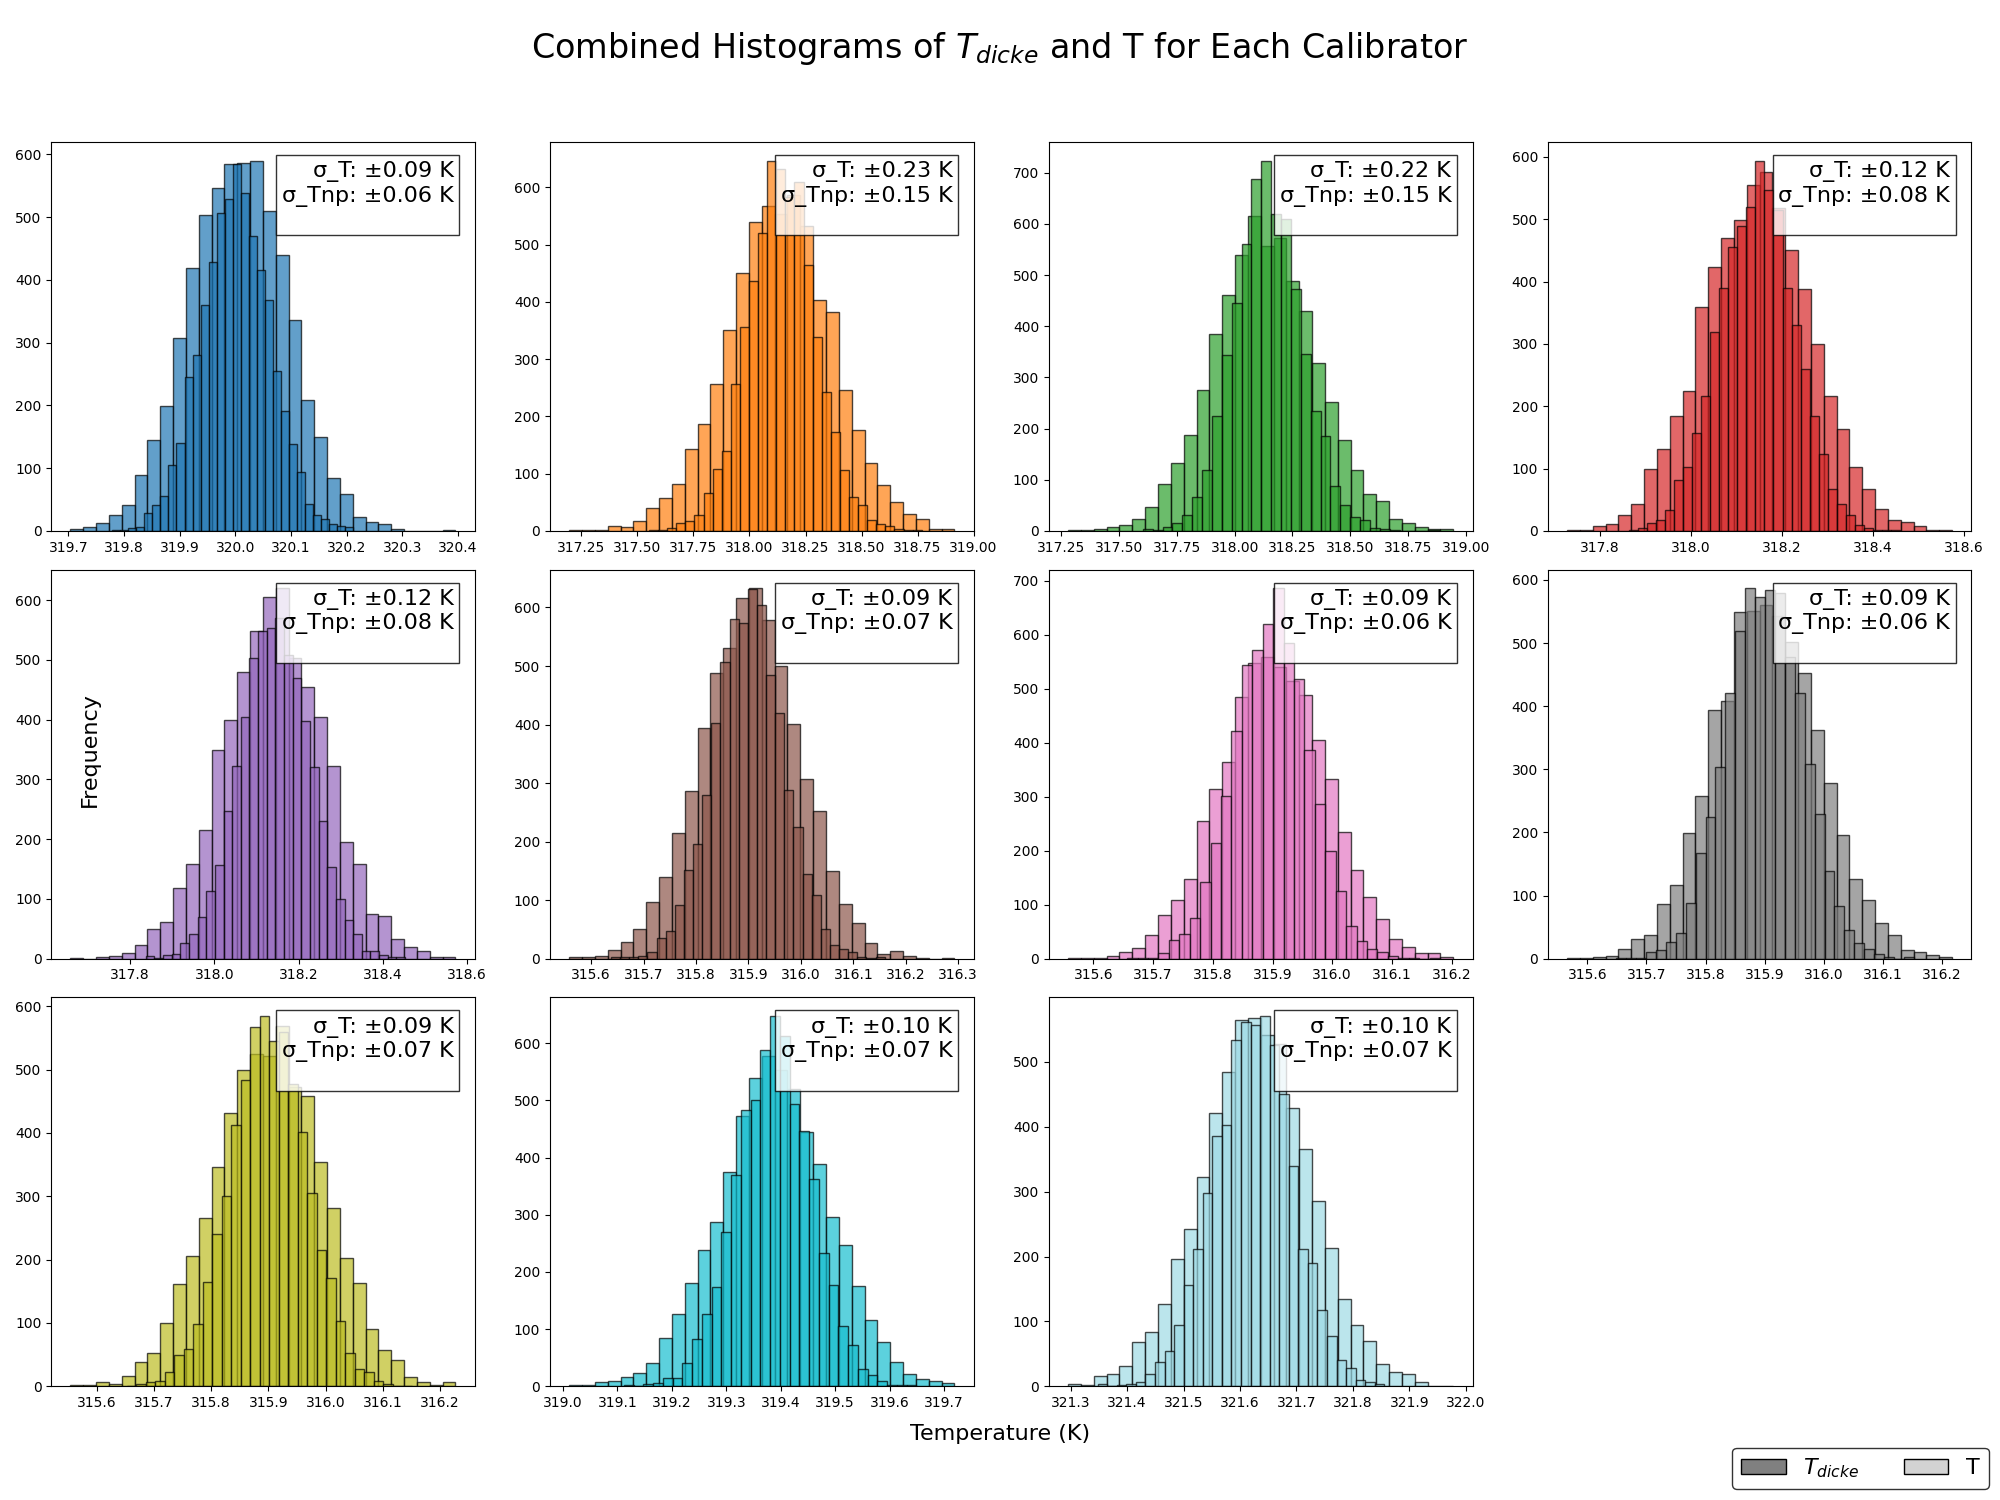
\includegraphics[width=0.9\textwidth]{images/combined_histograms.png}
			\end{figure}
		\end{column}
		\begin{column}{0.2\textwidth}
			Noise amplified by \textbf{30\%} when using
			\[
				T_{\text{NS}} \frac{P_{\text{cal}} - P_L}{P_{\text{NS}} - P_L} + T_L
			\]
		\end{column}
	\end{columns}
\end{frame}
\begin{frame}{\small{Why not fit noise (wave) parameters directly?}}

	% Noise Parameter Equation with smaller, uniform title
	\textbf{\small{Noise Parameter Equation:}}
	{\tiny
		\begin{equation}
			P_{\text{out}}^{\text{src}} = \textcolor{red}{g} M \left( T_{\text{in}}^{\text{src}} + \textcolor{red}{T_{\text{min}}} + T_0 \frac{4\textcolor{red}{R_N}}{Z_0} \frac{|\Gamma_{\text{src}} - \textcolor{red}{\Gamma_{\text{opt}}}|^2}{(1 - |\Gamma_{\text{src}}|^2)(1 + |\Gamma_{\text{opt}}|^2)} \right)
		\end{equation}
	}

	\vspace{0.05cm}
	\hrule  % Horizontal line for separation
	\vspace{0.05cm}

	% Noise Wave Equation with smaller, uniform title
	\textbf{\small{Noise Wave Equation:}}

	{\tiny
		\begin{multline}\label{}
			P_{\text{out}}^{\text{src}} = \textcolor{red}{g} \left[ \textcolor{red}{T_0} + \textcolor{red}{T_{\text{unc}}} |\Gamma_{\text{s}}|^2 \left|\frac{ \sqrt{1 - |\Gamma_{\text{rec}}|^2}}{1 - \Gamma_{\text{s}}\Gamma_{\text{rec}}} \right|^2 \right. \\
				\left. + T_{\text{s}}(1 - |\Gamma_{\text{s}}|^2) \left|\frac{ \sqrt{1 - |\Gamma_{\text{rec}}|^2}}{1 - \Gamma_{\text{s}}\Gamma_{\text{rec}}} \right|^2 + \textcolor{red}{T_{\text{cos}}} \Re \left( \Gamma_{\text{s}} \frac{\sqrt{1 - |\Gamma_{\text{rec}}|^2}}{1 - \Gamma_{\text{s}} \Gamma_{\text{rec}}} \right) \right. \\
				\left. + \textcolor{red}{T_{\text{sin}}} \Im \left( \Gamma_{\text{s}} \frac{\sqrt{1 - |\Gamma_{\text{rec}}|^2}}{1 - \Gamma_{\text{s}} \Gamma_{\text{rec}}} \right) \right]
		\end{multline}
	}

	\textit{We still end up with 5 unknowns, as before.}

\end{frame}


\end{document}
